


%% Los cap'itulos inician con \chapter{T'itulo}, estos aparecen numerados y
%% se incluyen en el 'indice general.
%%
%% Recuerda que aqu'i ya puedes escribir acentos como: 'a, 'e, 'i, etc.
%% La letra n con tilde es: 'n.

\chapter{Potenciales de corto alcance Darboux - deformados}

\section{Problema de partícula libre}

Para entender la utilidad de la transformación de Darboux degenerada en la construcción de estados ligados en el continuo, se estudia la deformación del potencial radial de partícula libre  $V=0 \; \forall r$ con momento angular $l=0$. En este caso, la correspondiente ecuación de Schrödinger $($con $ \frac{\hbar^2}{2m}=1$) es

\begin{equation*}
\frac{d^2 u}{dr^2} + k^2 u = 0,\,\,\,\, k^2 = E
\end{equation*}

Basándonos en la forma asintótica del ptencial que se quiere crear, se propone la siguiente solución particular como función de transformación

\begin{equation*}
u_T(q,r) = A(q) \sin[qr + \delta(q)]
\end{equation*}

Es decir, es una solución correspondiente al eigenvalor $E_q = q^2$. Para construir el potencial, el correspondiente wronskiano es de la forma

\begin{equation}
W_d = W[u_T,\partial_q u_T] =  \frac{1}{2}[\sin[2(qr+\delta)]-2q(r + \gamma_0)]. \label{WdPL}
\end{equation}

En este caso, se ha denotado \ref{WdPL} como tal debido a que es también la expresión correspondiente al denominador de las funciones transformadas. Sustituyéndolo en la fórmula $()$, se obtiene la expresión analítica para el potencial del nuevo sistema

\begin{equation*}
V_2 = 32 q^2   \frac{\sin\theta-q(r+\gamma_0)\cos\theta}{\sin(2\theta)-2q(r+\gamma_0)}\sin\theta
\end{equation*}

donde $qr + \delta = \theta, \,\,\,\, \gamma_0 =\partial_q \delta$


El potencial es del tipo von Neumann - Wigner, ya que su comportamiento asintótico es de la forma

\begin{eqnarray*}
	\lim_{r\rightarrow\infty} V_q^{(2)}(r) \rightarrow -4q\frac{\sin{2\theta}}{r}+O\left(\frac{1}{r^2}\right),
\end{eqnarray*} 

por lo tanto, la existencia de un estado ligado en el continuo es posible, de tal forma que éste correspondería a la energía $E=q^2$, el cual es precisamente el eigenvalor asociado a la función de transformación. Convenvcionalmente, de acuerdo al esquema de la transformación de Darboux, la función de transformación e mapeada a el caso trivial, sin embargo, al estar trabajando en el régimen continuo, se puede analizar lo que sucede en el límite $E \to q^2$, procedimiento a realizar en la subsección siguiente.


Para obtener el conjunto se doluciones del nuevo sistema, se realiza la transformación del par de soluciones linearmente independientes del sistema de partida $u^{\pm} = e^{\pm ikr}$, para lo cual se calcula el correspondiente wronskiano

\begin{equation*}
W^{\pm}_n= \frac{1}{2}  [2 q (k^2 - q^2)(r + \gamma_0) - (k^2 + q^2)\sin(2 \theta) \pm 4 i kq \sin^2 \theta ] e^{\pm i k r}
\end{equation*}

las soluciones del nuevo sistema están dadas por

\begin{equation}
\psi^{\pm}= \frac{2 q (k^2 - q^2)(r + \gamma_0) - (k^2 + q^2)\sin(2 \theta) \pm 4 i kq \sin^2 \theta }{\sin(2 \theta)-2q(r + \gamma_0)}e^{\pm i k r} \label{PSIPM}
\end{equation}

Al examinar el comportamiento asintótico de estas funciones

\begin{equation}
\psi^{\pm}|_{r \to \infty} = -(k^2 - q^2) e^{\pm ikr},\label{CAP}
\end{equation},

se observa que tienen el mismo comportamiento de las funciones de partida, con la diferencia de una factor poporcional. Podemos entonces escribir las soluciones de manera que (\ref{CAP}) sea de amplitud 1 (soluciones de Jost)

\begin{equation*}
f^{\pm} = -\frac{\psi^{\pm}}
{(k^2 - q^2)}
\end{equation*}

este análisis permite también observar que las funciones transformadas son linearmente independientes, por lo que la solución completa del sistema deformado como una combinación lineal de las funciones de Jost

\begin{equation}
\psi_s =A(k) f^{+}(k,r) + B(k) f^{-}(k,r) \label{CLSJ}
\end{equation}

Podemos entonces aplicar entonces la condición a la frontera propia de un problema radial dejando solo una constante arbitraria, la cual por conveniencia se define como $A=\frac{1}{2i}$

\begin{equation*}
\psi_s(k,0) = 0 \Longrightarrow \psi_s (k,r) = \frac{1}{2i} \left[f^{+}(k,r) - \frac{f^{+}(k,0)}{f^{-}(k,0)} f^{-}(k,r)\right]
\end{equation*}

para $\delta = 0$, usando identidades trigonométricas, se puede escribir $\psi_s$ como

\begin{equation*}
\psi_s(k,r) = \sin(kr) + 2 q \left\{ \frac{\sin[(k+q)r]}{k+q} - \frac{\sin[(k-q)r]}{k-q} \right\} \frac{\sin{qr}}{\sin(2qr) - 2q(r + \gamma_0)}
\end{equation*}

de está manera es fácil observar que el polo $-\frac{1}{(k^2 - q^2)}$ introduce una singularidad removible, por lo que se puede usar la regla de L'Hopital para obtener el límite cuando $k \to q$

\begin{equation*}
\psi_{bic}(q,r)=\lim_{k \to q}\psi_s(k,r) =  \frac{2 q \gamma_0 \sin(qr)}{\sin(2 qr) - 2q(r + \gamma_0)}
\end{equation*}

ya que el numerador en $\psi_b$ es acotado, para valores grandes de $r$, la funcion se desvanece, es decir, es una función de cuadrado integrable, y ya que $q > 0$, dicha función pertenece a la parte continua del espectro, por lo tanto es un estado ligado en el continuo.


Ya que un potencial de von Neumann Wigner está definido por su comportamiento asintótico, en la siguiente sección se propone extender el procedimiento realizado tomando como sistema de partida un potencial de corto alcance, ya que estos potenciales se comportan precisamente como un problema de partícula libre para valores muy grandes de $r$.

Aunque el objetivo principal de este trabajo es la construcción de sistemas que admitan la existencia de estados ligados en el continuo, la forma del potencial obtenido tiene regiones que cumplen con las condiciones necesarias para la existencia de estados ligados convencionales (véase figura $\ref{PPLTD}$). Podemos aplicar las condiciones a la frontera  vistas en la seccion  $\ref{SSELPCA}$ a la función $(\ref{CLSJ})$, quedando de la forma

\begin{equation*}
\psi_b = A \frac{2 q (\kappa^2 + q^2)(r + \gamma_0) - (\kappa^2 - q^2)\sin(2 \theta) + 4 \kappa q \sin^2 \theta }{\sin(2 \theta)-2q(r + \gamma_0)}e^{- \kappa r}.
\end{equation*}


Para obtener la condición de cuantización, aplicamos la condición a la frontera en el origen

\begin{equation*}
\psi_b|_{r=0} = 0 \Rightarrow 2 q \gamma_0 (\kappa^2 + q^2) - (\kappa^2 - q^2)\sin(2 \delta) + 4 \kappa q \sin^2 \delta = 0.
\end{equation*}

Para el caso $\delta = 0$, los términos que incluyen la función seno se anulan y la ecuación se reduce a

\begin{equation*}
\kappa^2 + q^2  = 0,
\end{equation*}

la cual no tiene soluciones en los números reales. Podemos concluir entonces que el potencial mostrado en la figura $\ref{PPLTD}$ no tiene estados ligados

\begin{figure}
	\centering
	\subfloat[]{\label{PPLTD}
		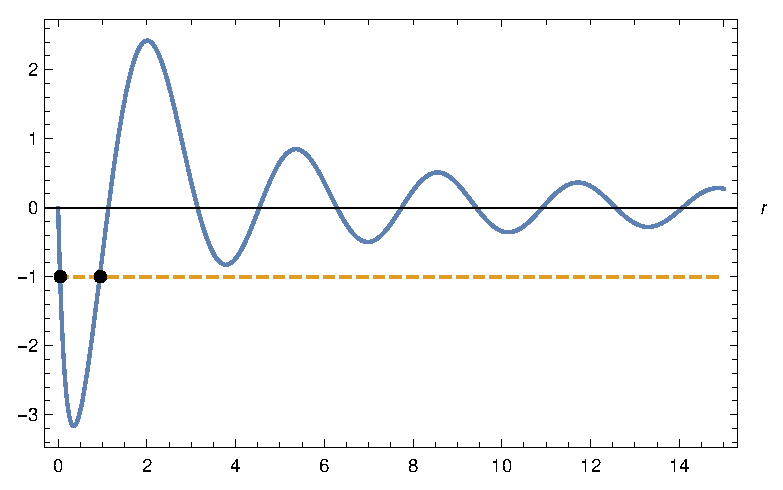
\includegraphics[width=0.42\textwidth]{PPLTD.eps}%
		\label{fig:a}%
	}%
	\hfill%
	\subfloat[]{%
		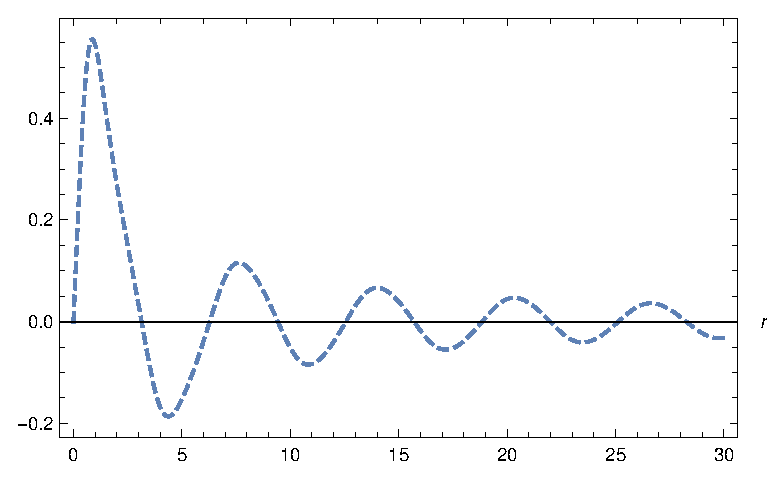
\includegraphics[width=0.42\textwidth]{PFOPLTD.eps}%
		\label{fig:b}%
	}%
	\caption{\label{PLTD-Figure} (a) Potencial de partícula libre deformado a partir de la transformación de Darboux degenerada (línea sólida) para $\delta = 0$ y $\gamma_0 = 1$. La línea punteada representa un hipotético valor para la energía perteneciente a un estado ligado. (b) Función de onda correspondiente al estado ligado en el continuo}
\end{figure}

\section{Potenciales de corto alcance Darboux - deformados}


Partiendo de un sistema cuyo potencial es de la forma $(\ref{PCA})$, el potencial en la región de interacción se toma como casi arbitrario, sólo exigienndo que su solución a la ecuación de Schrödinger sea puramente real

\begin{equation}
-\frac{d^2 u^{(i)}}{dr^2} + V^{(i)} u^{(i)} = E u^{(i)} : u^{(i)} \in \mathbb{R}.\label{eqRI}
\end{equation}

Lo siguente es elegir la función de transformación. Basado en el análisis de la sección anterior, dicha función es la siguiente

\begin{equation}
\label{FTAT}
u_T(q,r)=\begin{cases}
A(q)u^{(i)} (q,r) & r < R
\\\sin[qr+\delta(q)] & R < r
\end{cases}
\end{equation}

donde $u^{(i)}$ es solución a la ecuación $(\ref{eqRI})$. La continuidad de la función de transformación está contenida en el par de ecuaciones 

\begin{eqnarray}
\label{ccuT1}
A u^{(i)}(q,R)= \sin(qR + \delta)\\[0.3cm]
\label{ccuT2}
A \partial_r u^{(i)}(q,r)|_{r=R}= q\cos(qR + \delta).
\end{eqnarray} 

La función $(\ref{FTAT})$ y sus condiciones de continuidad tienen una  forma similar al caso de los estados ligados $(\ref{FOELPCA})$, por lo que se llega a la ecuación

\begin{equation*}
W[u^{(i)}(q,r), \sin(qr + \delta)]_{r = R} = 0,
\end{equation*} 
%Ressonances describes the pregerred way of decaying%
%Experimentally, they appear as sharp peaks in the cross section%
%Para ver los efec%
indicando que en un sistema con construido a través de la Transformación de Darboux degenerada con parámetro $R$ fijo, sólo para valores discretos de $q$ la función de transformación es continua y difrerenciable. Más aún, ya que las soluciones del nuevo sistema están dadas en términos de un wronskiano de tres funciones, sería necesaria la continuidad de la segunda derivada. La figura $\ref{}$ muestra la comparación entre una función transformada a partir de un valor del parámetro $q$ arbitrario y uno que cumple las condiciones necesarias para el caso del oscilador armónico truncado.

\begin{figure}
	\centering
	\subfloat[]{%
		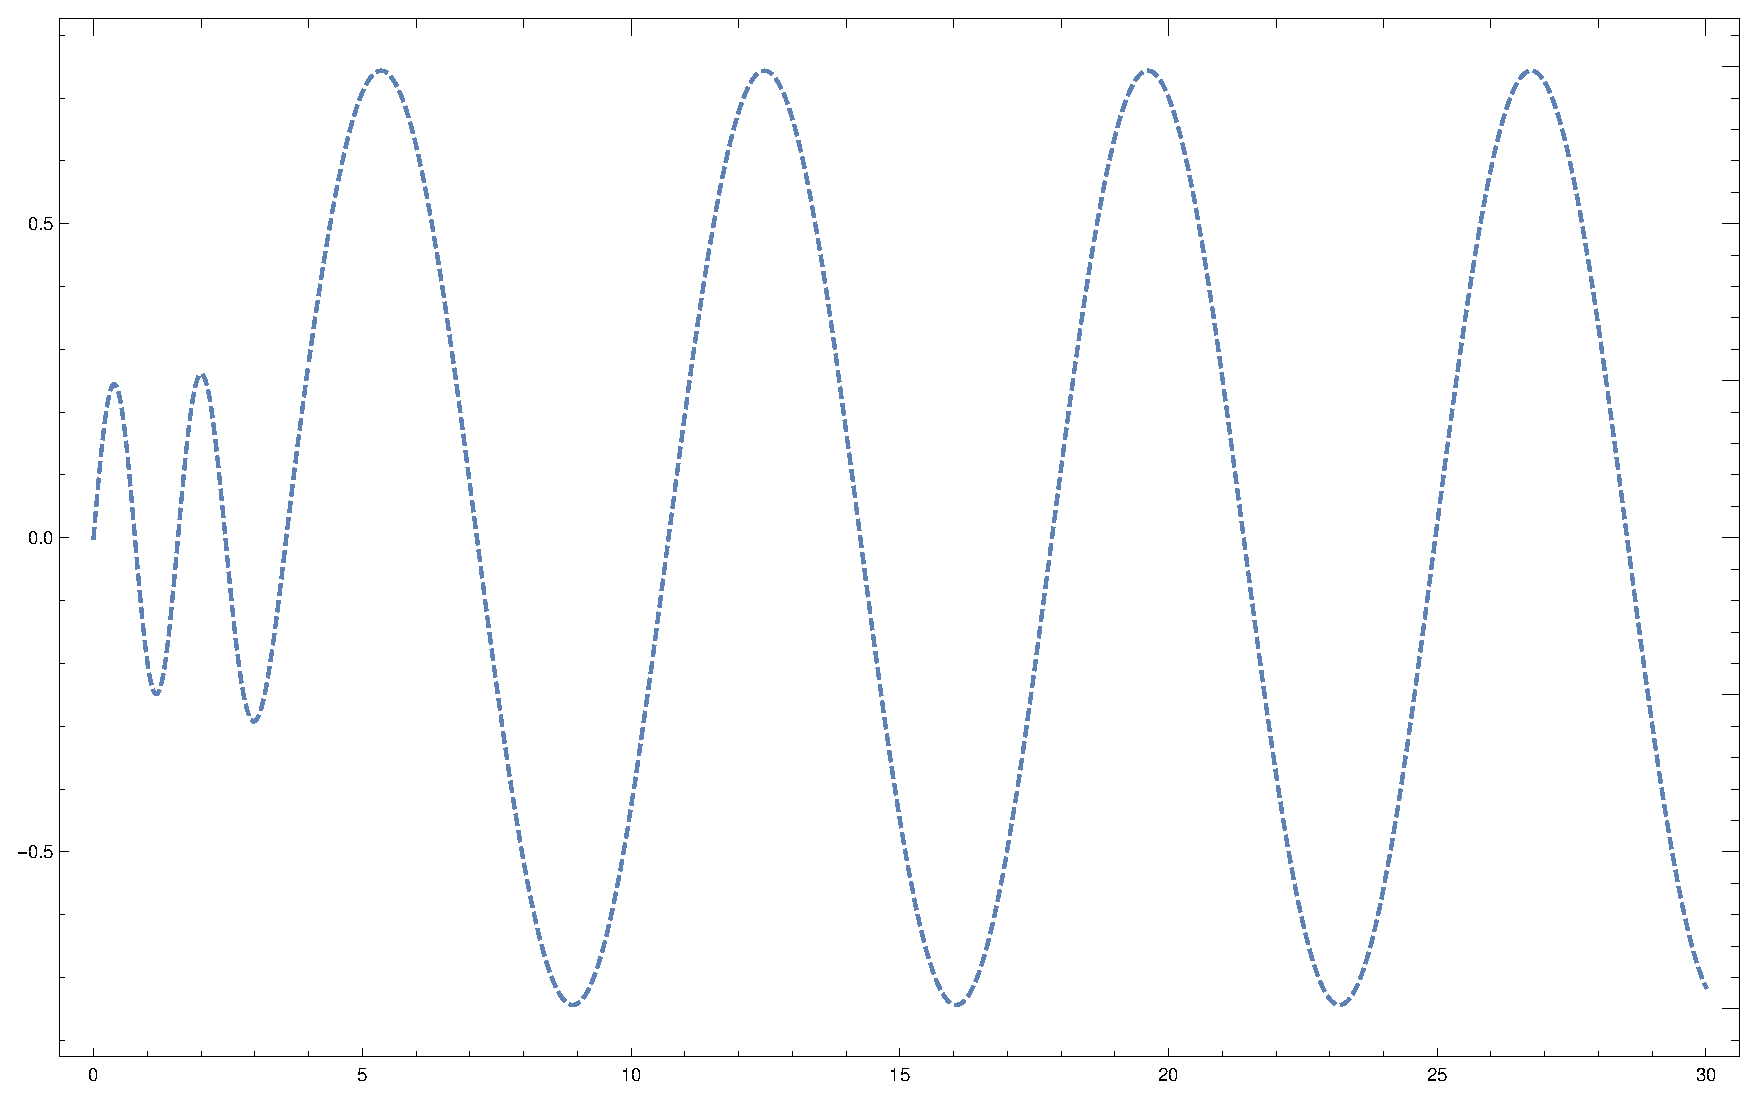
\includegraphics[width=0.41\textwidth]{Differentiable_transformation_function.eps}%
		\label{fig:a}%
	}%
	\hfill%
	\subfloat[]{%
		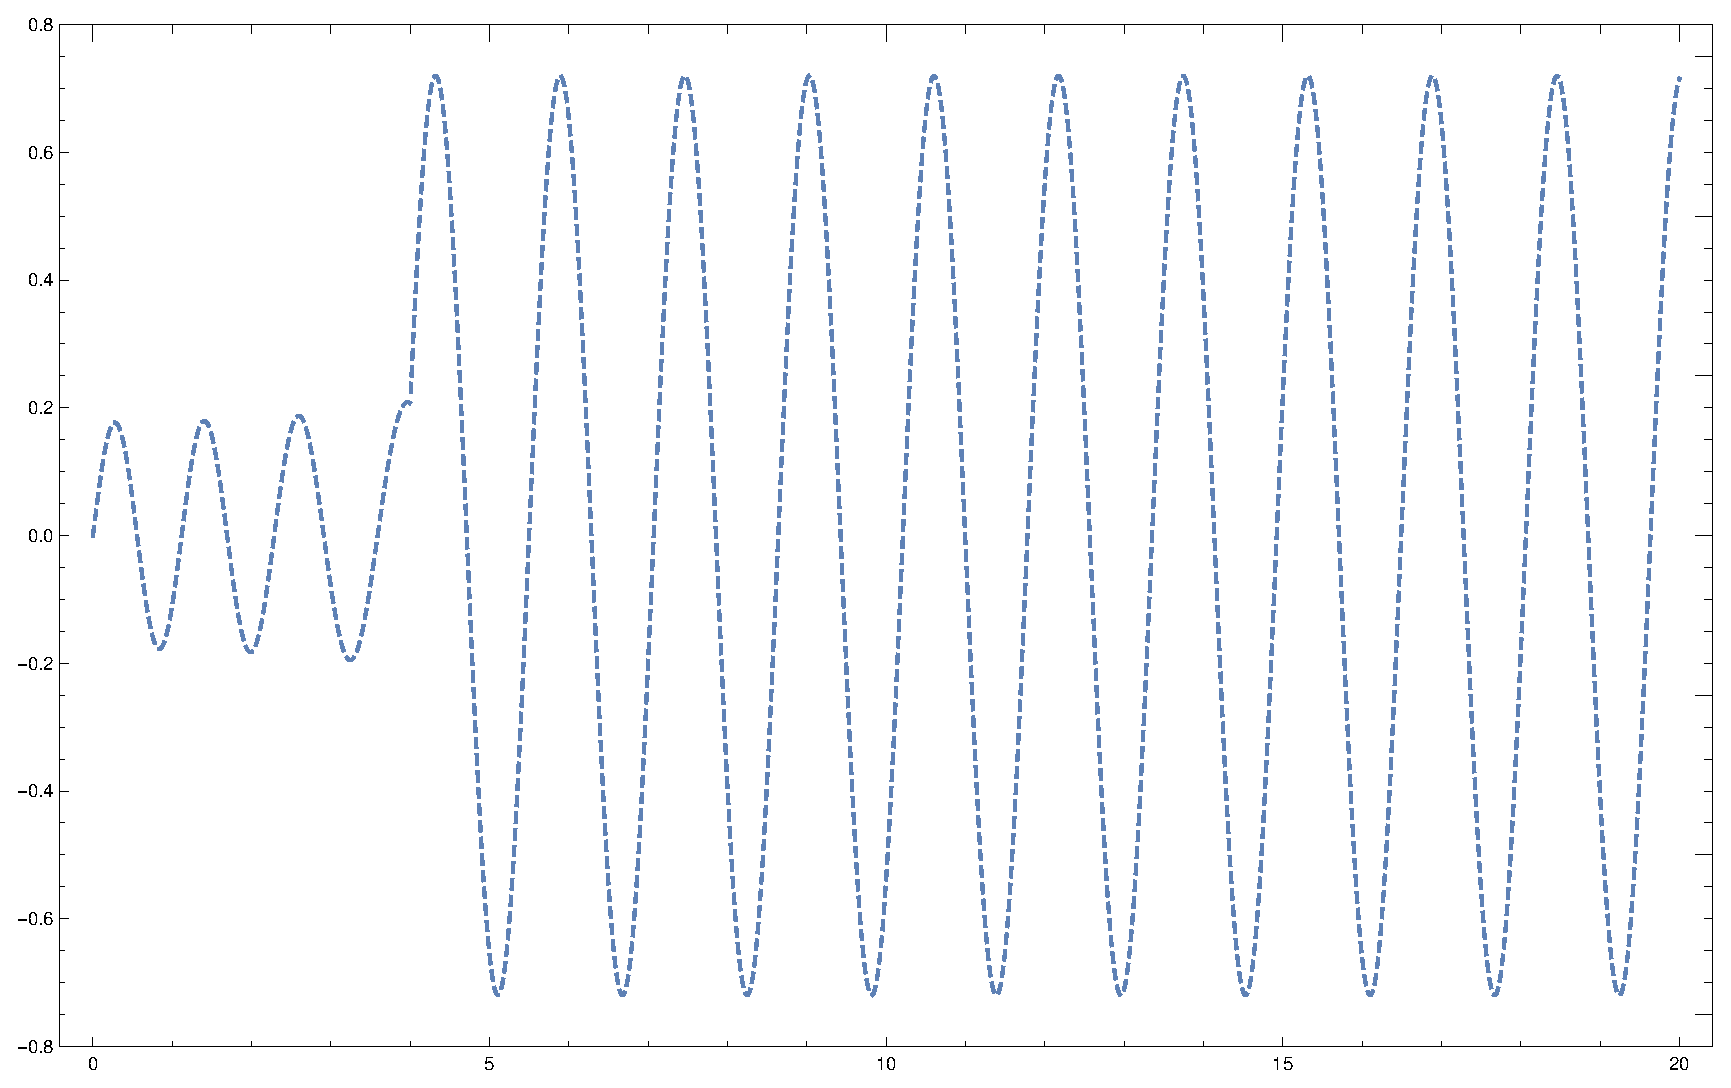
\includegraphics[width=0.41\textwidth]{Not_Differentiable_transformation_function.eps}%
		\label{fig:b}%
	}%
	\caption{\label{Figure CDNDTF} Funciones transformadas a partir del oscilador armónico truncado con un punto de corte $R=4$ como sistema inicial  y una  función de transformación con parámetros $\delta=0$, $\gamma_0 = 1$:  (a) Función continua y diferenciable con $q=0.880871$.
		b) Función continua pero no diferenciable con $q=4$ .}
\end{figure} 

Para evitar esta limitante, podemos observar que la función de transformación no es más que una herramienta matemática, ya que lo que realmente importa son las funciones y el potencial transformados. Se propone entonces transformar las soluciones del sistema inicial de manera independiente para cada región y después imponer las condiciones de continuidad en el nuevo sistema. En las siguientes subsecciones, se implementará dicho método, comenzando por asegurar que las funciones del sistema deformado sean regulares en el origen. 

\subsection{Comportamiento del sistema deformado en el origen}

Partiendo de un potencial de la forma $(\ref{PCAA})$ con la condicion previamente impuesta, se procede a realizar la transformación de Darboux para la función de onda en la región interna de acuerdo a la formula $()$. 

\begin{equation}
\psi^{(i)}(k,r) = \frac{W[u^{(i)}(q,r),\partial_q u^{(i)}(q,r),u^{(i)}(k,r)]}{W[u^{(i)}(q,r),\partial_q u^{(i)}(q,r)]} = \frac{W_n}{W_d}  \label{FITF}
\end{equation}

Al ser un problema radial, es importante garantizar que $\psi^{(i)}(k,r)|_{r=0}=0$, por lo que es natural pensar que esto se cumplirá al transformar soluciones al sistema inicial que sean regulares en el origen. Los dos sistemas a deformar en las secciones posteriores (oscilador armónico truncado y pozo radial) poseen la propiedad en la cual sus soluciones linearmente independientes tienen paridad definida, es decir

\begin{equation}
u^{(i)}(k,r) = A_i u^{(i)}_e (k,r) + B_i u^{(i)}_o (k,r)\label{FGSPD}
\end{equation}

donde $u^{(i)}_e$ tiene paridad par y $u^{(i)}_o$ es una función impar. Por lo tanto, la solución que es regular en el origen es la de paridad impar. Sean entonces  $u(E_k,r)$ y $u(E_q,r)$  soluciones a una ecuación de Schrödinger con paridad par. Los wronskianos correspondientes a la función transformada en el origen son


\begin{eqnarray*}
& W_n |_{r=0}= Det\, 
\begin{pmatrix}
0 & 0 & 0
\\
\partial_r u(E_q,0) & \partial_r \partial_E u(E_q,0) & \partial^2_r u(E_k,0)
\\
\partial^2_r u(E_q,0) & \partial^2_r \partial_E u(E_q,0) & \partial^2_r u(E_k,0)

\end{pmatrix} = 0
\\[0.4cm]
& W_d |_{r=0}= Det\, 
\begin{pmatrix}
0 & 0
\\
\partial_r u(E_q,0) & \partial_r \partial_E u(E_q,0)
\end{pmatrix} = 0
\end{eqnarray*}

Entonces podemos usar la regla de L'Hopital para obtener la forma de las soluciones al nuevo sistema en el origen. Con este fin, es  importante tomar en cuenta lo siguiente:

La posición y la energía son variables independientes, por lo que es equivalente el evaluar la función en $r$ y posteriormente derivar con respecto a $E$ o viceversa

\begin{equation*}
[\partial_E \partial_r u(E,r)]_{r=0} =  \partial_E [\partial_r u(E,r)|_{r=0}] 
\end{equation*}

Al ser $u(E,r)$ solución a la ecuación de Schrödinger, su segunda derivada con respecto a la posición en el origen es

\begin{equation}
-\partial^2_r u(E,r)|_{r=0} =  [E-V(0)]u(E,0) \label{ESIEO},
\end{equation}

y al derivar la expresión anterior con respecto a $E$ se obtiene

\begin{equation}
-\partial_E \partial^2_r u(E,r)|_{r=0} = u(E,0)+ [E-V(0)] \partial_E u(E ,0) \label{DEESIEO}.
\end{equation}

Además, ya que $u_e$ y $u_0$ son linearmente indepedientes, el wronskiano es diferente de cero para todo $r$, incluyendo el origen \cite{WronskianP}

\begin{equation}
W[u_e(E,r), u_o(E,r)]_{r=0} = [u_e(E,r)\partial_r u_o(E,r) - u_o(E,r)\partial_r u_e(E,r)]_{r=0} \ne 0 \label{PW1}
\end{equation}

En el caso de la función impar, las condiciones anteriores implican que

\begin{eqnarray*}
\partial^2_r u_o(E,r)|_{r=0} = \partial_E \partial^2_r u_o(E,r)|_{r=0} = 0
\\
\partial_r u_o(E,r)|_{r=0} \ne 0
\end{eqnarray*}

Las propiedades anteriores implican que es necesario usar L'Hopital tres veces, por lo que la expresión final es

\begin{equation*}
\lim_{r \to 0} \frac{W_n}{W_d} = \frac{\lim_{r \to 0} \partial^3_r W_n}{\lim_{r \to 0} \partial^3_r W_d} = \frac{0}{[-\partial_r u_o(E,r)|_{r=0}]^2} = 0
\end{equation*}

Efectivamente, si se usa una solución impar (regular en el origen) como función de transformación para transformar soluciones de la misma paridad, se obtiene una función regular en el origen. 

El resultado anterior, junto con el hecho de que la herramienta de la transformación de Darboux permite usar soluciones "no físicas" tanto como función de transformación o función a transformar (caso de "missing states"), nos invita a explorar el caso en el que partimos de un conjunto de soluciones a la ecuación de Schrödinger $u(E,r)$ con paridad par e irregulares en el origen

\begin{equation*}
u(E,r)|_{r=0} \ne 0,
\end{equation*}

donde además, al ser su derivada de paridad par 

\begin{equation*}
\partial_r u(E,r)|_{r=0} = 0,
\end{equation*}

por lo que en este caso los wronskianos correspondientes a las funciones transformadas en el origen son

\begin{eqnarray*}
	& W_n |_{r=0}= Det\, 
	\begin{pmatrix}
		u(E_q,0) & \partial_E u(E_q,0) & \partial^2_r u(E_k,0)
		\\
		0 & 0 & 0
		\\
		\partial^2_r u(E_q,0) & \partial^2_r \partial_E u(E_q,0) & \partial^2_r u(E_k,0)
		
	\end{pmatrix} = 0
	\\[0.4cm]
	& W_d |_{r=0}= Det\, 
	\begin{pmatrix}
		\partial_r u(E_q,0) & \partial_r \partial_E u(E_q,0)
		\\
		0 & 0
	\end{pmatrix} = 0
\end{eqnarray*}

Entonces, al igual que en el caso anterior, podemos usar L'Hopital en $r \rightarrow 0$, donde las propiedades $(\ref{ESIEO})$ y($\ref{DEESIEO}$) implican que

\begin{equation*}
\lim_{r \to 0} \frac{W_n}{W_d} = \frac{\lim_{r \to 0} \partial_r W_n}{\lim_{r \to 0} \partial_r W_d} = \frac{0}{[-u_e(E,r)|_{r=0}]^2} = 0
\end{equation*}

Podemos decir entonces que la transformación de Darboux degenerada permite obtener soluciones regulares en el origen si se toma una función con paridad definida como función de transformación y se transforman funciones de la misma paridad. 

Más aún, podemos analizar un tercer caso, aquel donde la función de transformación es una combinación lineal de las dos soluciones linealmente independientes a la misma ecuación de Schrödinger con paridad definida

\begin{equation*}
u^{(i)}_T (E_q,r) = \alpha_1(E_q) u^{(i)}_e(E_q,r) + \beta_1(E_q) u^{(i)}_o(E_q,r),
\end{equation*}

y la derivada con respecto a la energía es de la forma

\begin{equation*}
\partial_E u^{(i)}_T (q,r) = \alpha_2(E_q) u^{(i)}_e(E_q,r) + \beta_2(E_q) u^{(i)}_o(E_q,r) +  \alpha_1(E_q) \partial_E u^{(i)}_e(E_q,r) + \beta_1(E_q) \partial_E u^{(i)}_o(E_q,r),
\end{equation*}
 
donde $\alpha_2 = \partial_E \alpha_1 $ y $\beta_2 = \partial_E \beta_1 $. El sistema creado tendrá pues seis parámetros, cuatro para la región interna y dos para la región externa. Las funciones transformadas que componen al nuevo sistema son

\begin{eqnarray*}
\psi^{(i)}_{e}(k,r) = \frac{W[ u^{(i)}_T (E_q,r),\partial_E u^{(i)}_T (E_q,r),u_e(E_k,r)]}{W[ u^{(i)}_T (E_q,r),\partial_E u^{(i)}_T (E_q,r)]} = \frac{W_{ne}}{W_d}
\\
\psi^{(i)}_{o}(k,r) = \frac{W[ u^{(i)}_T (E_q,r),\partial_E u^{(i)}_T (E_q,r),u_o(E_k,r)]}{W[ u^{(i)}_T (E_q,r),\partial_E u^{(i)}_T (E_q,r)]} = \frac{W_{no}}{W_d}
\end{eqnarray*}

 Mediante las mismas propiedades que se usaron en los casos con paridad definida, podemos evaluar los wronskianos correspondientes en el origen

\begin{eqnarray*}
W_{ne}|_{r=0} &=& W[ u^{(i)}_T (E_q,r),\partial_E u^{(i)}_T (E_q,r),u_e(E_k,r)]|_{r=0}
\\
&=& u^{(i)}_e(E_k,0)\{(E_q - E_k)u_e^{(i)}(E_q,0)[(\alpha_2 \beta_1 - \alpha1 \beta_2)\partial_r u_o^{(i)}(E_q,0) - \alpha_1 \beta_1 \partial_E \partial_r  u^{(i)}_o(q,0)]
\\
&-& \alpha_1 \beta_1 \partial_r  u^{(i)}_o(E_q,0)[(E_k - V(0))\partial_E u^{(i)}_e(E_q,0) + \partial_E \partial^2_r u^{(i)}_e(E_q,0)]\}
\end{eqnarray*}

\begin{equation*}
	W_{no}|_{r=0} = \alpha^2_1 [u^{(i)}_e(E_q,0)]^2 \partial_r u^{(i)}_o(E_k,0)
\end{equation*}

\begin{eqnarray*}
W_{d}|_{r=0} &=& -\partial_r u^{(i)}_o(E_q,0)[u^{(i)}_e(E_q,0)(\alpha_2 \beta_1 - \alpha_1 \beta_2) 
\\
&+& \alpha_1 \beta_1 \partial_E u^{(i)}_e(E_q,0)] + \alpha_1 \beta_1 u^{(i)}_e(E_q,0) \partial_r \partial_E u^{(i)}_o(E_q,0)
\end{eqnarray*}

Suponiendo que los valores de los parámetros son tales que $W_{ne}|_{r=0}$,  $W_{ne}|_{r=0}$ y $W_{d}|_{r=0}$ sean diferente de cero, entonces podemos construir la solución completa al nuevo sistema por medio de la combinación lineal

\begin{equation*}
\psi^{(i)}(k,r) = A_i \psi^{(i)}_{e}(k,r) + B_i \psi^{(i)}_{o}(k,r),
\end{equation*}

y aplicando la condición a la frontera de un problema radial, pudemos escribir

\begin{equation*}
\psi^{(i)}(k,r) = A_i \left[\psi^{(i)}_{e}(k,r) - \frac{W_{ne}|_{r=0}}{W_{no}|_{r=0}} \psi^{(i)}_{o}(k,r)\right], 
\end{equation*}

de esta forma, la función $\psi^{(i)}(k,r)$ es regular en el origen. La figura muestra un ejemplo de este caso, en donde el sistema inicial es el pozo radial

\begin{figure}
	\centering
	\subfloat[]{%
		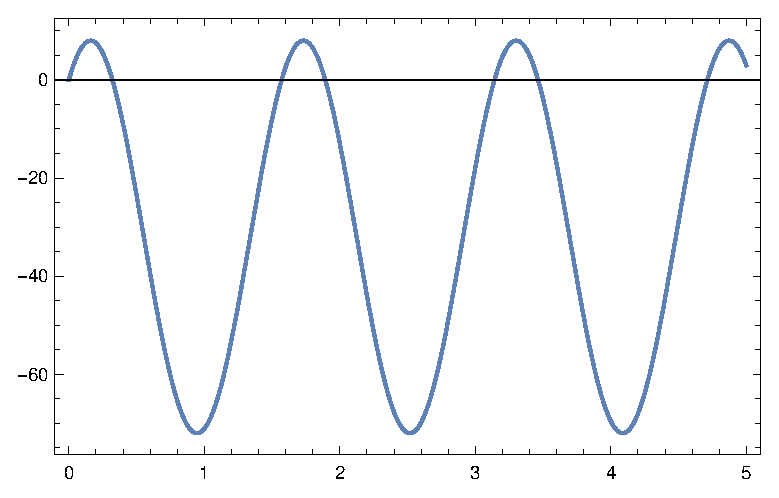
\includegraphics[width=0.41\textwidth]{PTDCL.eps}%
		\label{fig:a}%
	}%
	\hfill%
	\subfloat[]{%
		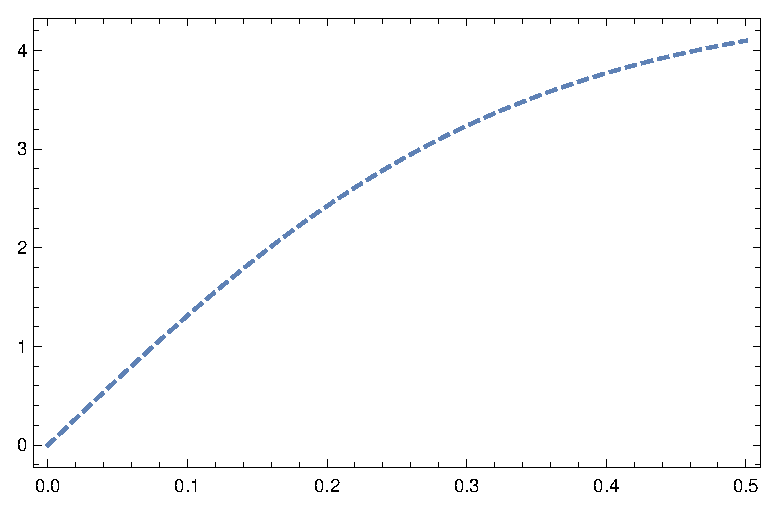
\includegraphics[width=0.41\textwidth]{FOOTDCL.eps}%
		\label{fig:b}%
	}
	\caption{\label{Fig_POAEO} 
		Potencial creados a partir la región de interacción de un pozo radial con profundidad $3$ y una combinación lineal de sus soluciones linealmente independientes. Solucion (b) cerca del origen para los valores de parametros $\alpha_1 = 1,\, \beta_1 = 2,\, \alpha_2 = 3,\, \beta_2 = 4$}
\end{figure} 




Por otro lado, partiendo de un potencial de la forma $(\ref{PCAA})$, su deformación por medio de la transformación de Darboux degenerada en la región interna es de la forma

\begin{equation}
V_2^{(i)}(r) = V^{(i)} - 2 \frac{(\partial_r W_d)^2 - W_d \partial^2_r W_d}{W_d^2} \label{PDTWd}
\end{equation}

Donde se ha desarrollado la parte que contiene la deformación en términos del denominador en la expresión $(\ref{FITF})$, con el fin de conocer lo que ocurre en el origen por medio de lo estudiado anteriormente, este comportamiento es de la forma

\begin{equation*}
\lim_{r \to 0} V_2^{(i)}(r) \rightarrow \infty.
\end{equation*}

Esto sucede tanto en la versión regular como en la versión irregular de la transformación. Sin embargo, a pesar de que el potencial construido es singular en el origen, esta singularidad no es heredada por las soluciones, la figura $(\ref{Fig_POAEO})$ muestra dos potenciales creados a partir del oscilador armónico y una solución par e impar.

\begin{figure}
	\centering
	\subfloat[]{%
		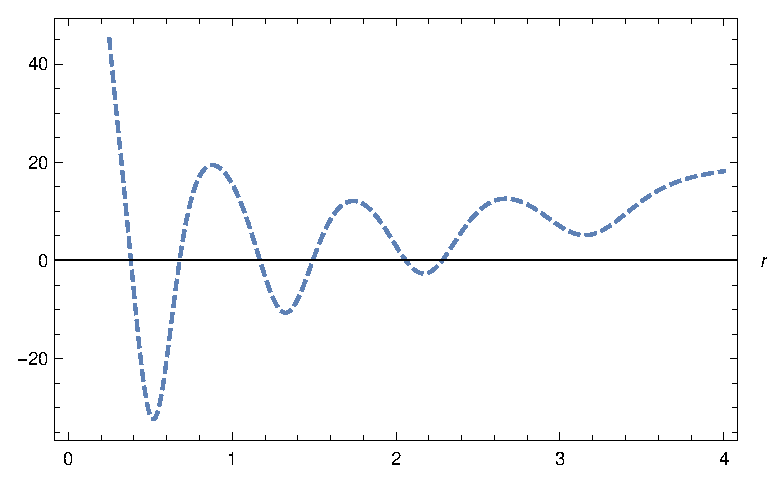
\includegraphics[width=0.41\textwidth]{PPOATTDe.eps}%
		\label{fig:a}%
	}%
	\hfill%
	\subfloat[]{%
		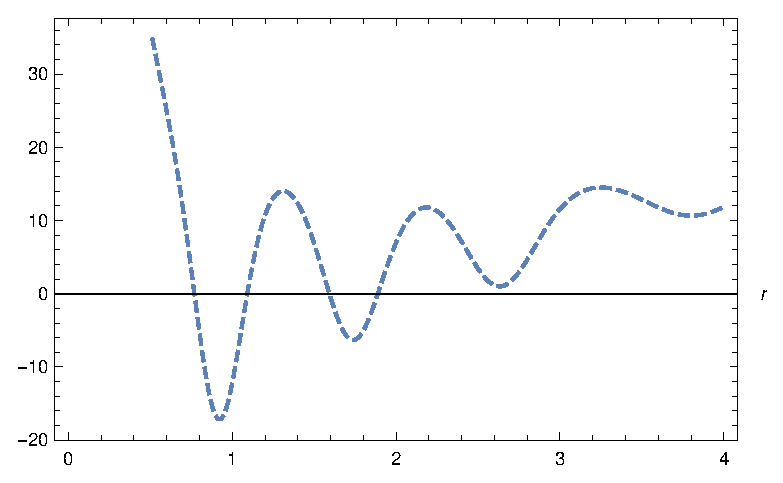
\includegraphics[width=0.41\textwidth]{PPOATTDo.eps}%
		\label{fig:b}%
	}
	\hfill%
	\subfloat[]{%
		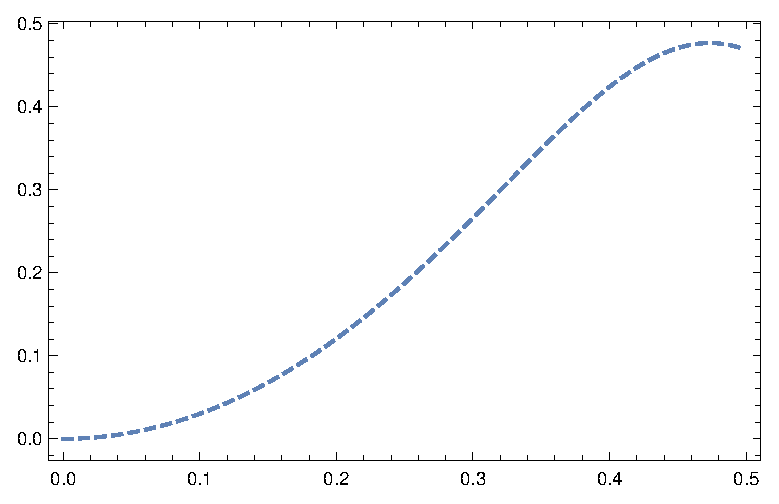
\includegraphics[width=0.41\textwidth]{FOTDe.eps}%
		\label{fig:c}%
	}
	\hfill%
	\subfloat[]{%
		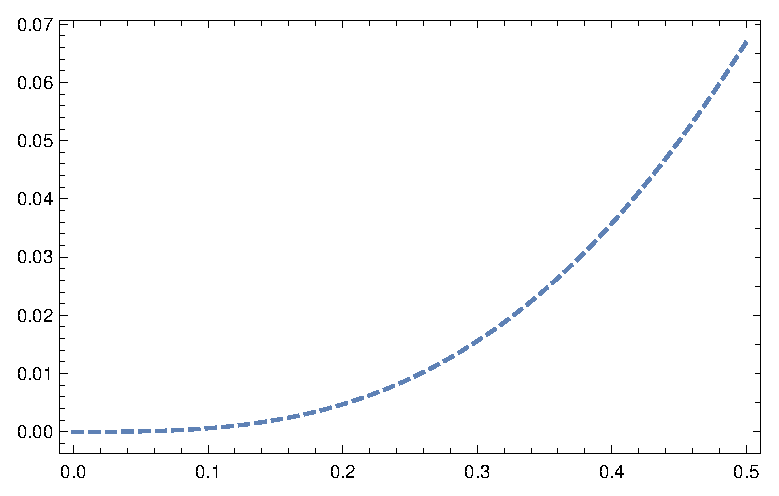
\includegraphics[width=0.41\textwidth]{FOTDo.eps}%
		\label{fig:c}%
	}
	\caption{\label{Fig_POAEO} 
		Potenciales creados a partir del oscilador armónico y una solución (a)par e (b) impar con sus respectivas soluciones (c) y (d)}
\end{figure} 

Ahora que ha sido satisfecha la condición a la frontera para un problema radial deformado por medio de la transformación degenerada de Darboux cuyo sistema de partida tiene características que cumplen tanto el pozo radial como el oscilador armónico truncado, podemos proceder a analizar el sistema de llegada de manera general, comenzando por construir la parte discreta del espectro.



%%%%%%%%%%%%%%%%%%%%%%%%%%%%%%%%%%%%%%%%%%%%%%%%%%%%%%%%%%%%%%%%%%%%%%%%%%%%%%%%%%%%%%%%%%%%%%%%%%%%%%%%%%%%%%%%%%%%%%%%%%%%%%%%%%
\subsection{Potencial radial Darboux - deformado}
%%%%%%%%%%%%%%%%%%%%%%%%%%%%%%%%%%%%%%%%%%%%%%%%%%%%%%%%%%%%%%%%%%%%%%%%%%%%%%%%%%%%%%%%%%%%%%%%%%%%%%%%%%%%%%%%%%%%%%%%%%%%%%%%%%

Partimos de un potencial de la forma 

\begin{equation}
V_2 = 
\begin{cases}
V_2^{(i)}(r) & r < R
\\
32 q^2   \frac{\sin\theta-q(r+\gamma_0)\cos\theta}{\sin(2\theta)-2q(r+\gamma_0)}\sin\theta & R < r \label{PDDG}
\end{cases},
\end{equation}
donde $V^{(i)}$ es un potencial de la forma $(\ref{PDTWd})$, es decir, es un potencial deformado por medio de la solución (\ref{FGSPD}). Por otro  lado, en la región externa, tenemos el potencial construido en la subsección anterior a partir del sistema de partícula libre.


De forma general, la función de onda completa es de la forma $(\ref{FITF})$

\begin{equation}
\psi_s(r)=\begin{cases}
A_i \psi^{(i)}(k,r) & r < b
\\\ B_e \psi^{+}(k,r) + C_e \psi^{-}(k,r) & b < r.
\end{cases},\label{FOGC}
\end{equation}

dode  $\psi^{(i)}$ es construida a partir de (\ref{FITF}), por lo que que la regularidad en el origen está garantizada, mientras que $\psi^{\pm}$ esta dada por (\ref{PSIPM}). La expresión (\ref{FOGC}) permite obtener los estados ligados y de dispersión del sistema aplicando las condiciones a la frontera pertinentes.


\subsection{Estados ligados}

El comportamiento asintótico de  \ref{PDDG} nos dice que los estados ligados se dan para valores de la energía $E < 0$, lo que implica un valor de $k$ puramente imaginario, es decir, $k = i \kappa : \kappa \in \mathbb{R}$. La expresión asintótica de $(\ref{FOGC})$ toma la forma

\begin{equation}
\psi_s(r)|_{r \to \infty} = B_e e^{-\kappa r} + C_e e^{\kappa r}
\end{equation}

por lo que si $\kappa > 0$, para que la función de onda sea de cuadrado integrable, el coeficiente $C_e$ debe ser igual a cero. Además, como cualquier problema dividido en regiones, lo siguiente es garantizar la continuidad y diferenciabilidad de las eigenfunciones, lo cual se cumple mediante el par de ecuaciones
\begin{eqnarray}
A_i \psi^{(i)}(i\kappa,b)= B_i \psi^{+}(i\kappa,b) \\[0.3cm]\label{ELC1}
A_i \partial_r \psi^{(i)}|_{r=b,k=i\kappa}= B_i \partial_r\psi^{+} |_{r=b,k=i\kappa} \label{ELC2}.
\end{eqnarray} 

El coeficiente $A_i$ de deja como constante de normalización, mientras que $B_e$ se obtiente mediante $(\ref{ELC1})$, quedando la función de onda de la forma
\begin{equation*}
A_i
\psi_s(r)=\begin{cases}
\psi^{(i)}(i \kappa,r) & r < R
\\\ \frac{\psi^{(i)}(i \kappa,R)}{\psi^{+}(i \kappa,R)} \psi^{+}(i \kappa,r) & R < r
\end{cases}
\end{equation*}

 y al sustituir el valor de $B_e$ en $(\ref{ELC2})$, se llega a la ecuación trasendental

\begin{equation}
W[\psi^{(i)},\psi^{+}]_{r=R, k = i \kappa}=0 \label{CCG}
\end{equation}


Al resolver $(\ref{CCG})$ para $\kappa^2 = |E|$, se obtienen los valores de la energía para los cuales $\psi_s$ es de cuadrado integrable, generando un espectro discreto correspondiente a los estados ligados. Al contar con esta parte del espectro el sistema construido es uno más completo que los propuestos en las secciones anteriores. En la siguiente sección se construirá el espectro continuo del sistema utilizando la forma general de la función de onda.


\subsection{Espectro de dispersión}


El caso del régimen de la dispersión está compuesto por los eigenvalores de la energía $k^2 = E >0$ correspondientes a eigenfunciones acotadas dadas por $(\ref{FOGC})$, formando un espectro continuo. La continuidad y diferenciabilidad de las funciones es garantizada por las ecuaciones correspondientes


\begin{eqnarray*}
A_i \psi^{(i)}(k,R) = [B_e \psi^{+} + C_e \psi^{-}]_{r=R}\\
A_i \partial_r \psi^{(i)}|_{r=R}= [B_e \partial_r \psi^{+} + C_e \partial_r \psi^{-}]_{r=R}
\end{eqnarray*} 

Las combinación lineal de funciones con la forma asintótica (\ref{CAP}) cumplen con la siguiente simetría en sus coeficientes, siempre que la funcion en la región interna sea puramente real

\begin{equation}
B_e = -C_e^{*},\,\,\,\, B_e = A_i \frac{W[\psi^{(i)},\psi^{-}]}{W[\psi^{+},\psi^{-}]} \label{CSS}
\end{equation}

Ahora que se han construido las soluciones de la dispersión, se realizará un análisis de la solución de la dispersión correspondiente a el valor de la energía $k \to q$, el cual según el la forma asintótica del potencial puede corresponder a un estado ligado en el continuo.

\subsection{Estado ligado en el continuo}

De acuerdo al esquema de la transformación de Darboux, la solución asociada a la energía correspondiente a $E=q^2$ es mapeada al caso trivial, pero como se demostró al usar la transformación de Darboux degenerada para el caso de partícula libre, es posible realizar un análisis en el límite $k \to q$ mediante la introducción de un polo en dicho valor mediante la constante arbitraria. Sin enbargo, debido a la forma de $\psi^{(i)}$, se cumple además que $\partial_k \psi^{(i)}|_{k=q}=0$, por lo que el polo a introducir debe ser de segundo orden. En este caso se ha elegido que la función en la región interna sea de la forma

\begin{equation*}
A \psi^{(i)} = A' \frac{\psi^{(i)}(k,r)}{\psi^{(i)}(k,R)},
\end{equation*}

esto debido a que el polo se comporta de la misma manera que $\psi^{(i)}(k,r)$ con respecto a $k$. Ya que hemos obtenido una forma adecuada para la función de onda, además de el valor de los coeficientes que hacen que la función de onda sea continua, ahora estamos en condiciones de realizar el análisis en $k \to q$, para lo cual es conveniente escribir la función de onda de la siguiente manera gracias a $(\ref{CSS})$


\begin{equation}
\psi_s(k,r)=A' \begin{cases}
\frac{\psi^{(i)}(k,r)}{\psi^{(i)}(k,R)} & r < R
\\ \frac{Im[W(\psi^{(i)},\psi^{-})_{r=R}\psi^{-}(k,r)]}{\psi^{(i)}(k,R) Im [\psi^{+} \partial_r \psi^{-}]_{r=R}} & R < r
\end{cases}
\label{FOPCADD}
\end{equation}

La introducción del polo permite el uso de la regla de L'Hopital en el límite deseado. Para la región de interna, la función toma la forma 

\begin{equation*}
\lim_{k \to q} A' \frac{\psi^{(i)}(k,r)}{\psi^{(i)}(k,R)} =  A' \frac{\partial^2_k \psi^{(i)}|_{k=q}}{\partial^2_k \psi^{(i)}|_{k=q,r=R}}
\end{equation*}


Por otro lado, en la región $R < r$ al observar el comportamiento de $\psi^{\pm}$ en el límite

\begin{equation*}
Im[\psi^{\pm}]_{k=q} =0\, \Longrightarrow Im [\psi^{+} \partial_r \psi^{-}]_{k=q} = 0
\end{equation*}


podemos notar que la presencia del polo provoca que el cero tanto en el numerador como en el denominador en (\ref{FOPCADD})  para $b < r$ sean de cuarto aorden. Como consecuencia, en este caso la regla de L'Hopital debe ser usada en cuatro ocasiones. Después de este procedimiento, debido a la complejidad de la expresión resultante, es más conveniente analizar el numerador  y denominador por separado


\begin{equation*}
\lim_{k \to q} A' \frac{Im[W(\psi^{(i)},\psi^{-})_{r=b}\psi^{-}(k,r)]}{\psi^{(i)}(k,r)|_{r=b} Im [\psi^{+} \partial_r \psi^{-}]_{r=b}} = \frac{f_n(q,b,r)}{f_d(q,b,r)}.
\end{equation*}

Donde el numerador es de la forma

\begin{eqnarray*}
	f_n(q,R,r)&=& W \left\{\partial^2_k\psi^{(i)}(k,r), {\rm Re}[\psi^{+} (k,r)]\right \}_{k = q, r = R} \,g_1(q,r)\\[0.2cm]
	&+&2 W \left\{\partial^2_k\psi^{(i)}(k,r), \partial_{k}{\rm Im}\left[\psi^{+}(k,r)\right] \right\}_{k=q,r=R}\, g_2(q,r)\\[0.2cm]
	&+&\frac{2}{\gamma_0} W \left\{ \partial^2_k \psi^{(i)}(k,r), \partial_{k}{\rm Re}\left[\psi^{+}(k,r)\right]\right\}_{k=q,r=R} \,g_3(q,r)\\[0.2cm]
	&+& W \left\{ \partial^2_{k}\psi^{(i)}(k,r),\partial^2_k {\rm Im}\left[\psi^{+}(k,r)\right] \right\}_{k=q, r=R}\, g_3(q,r).
\end{eqnarray*}

mientras que las funciones $g_i(q,r)$, están dadas por

\begin{eqnarray*}
	g_1(q,r)&=&\frac{(2 \sin{qr} - 2r ) \sin{[2 (q r + \delta)]} - 
		2 q (q r (3 r + 4 \gamma_0) \cos{qr} + 
		q r^2 \cos{[2 (q r + \delta)]} + 2 \gamma_0 \sin{qr}}{\sin{2qr}-2q(r+\gamma_0)}\\[0.2cm] 
	g_2(q,r)&=& 2q \frac{q(r + 2 \gamma_0) \cos{qr} + qr \cos{[2(qr + \delta)]} - 
		2\cos{\delta} \sin{(q r + \delta)}}{-2q(\gamma_0+r)+\sin{[2(qr+\gamma_0)]}},\\[0.2cm] 
	g_3(q,r)&=&\frac{2q\sin{(qr + \delta)}}{\sin{[2(qr+\delta)]}-2q(r+\gamma_0)}. 
\end{eqnarray*}

y su comportamiento asintótico es de la forma

\begin{eqnarray*}
	\lim_{r\rightarrow\infty}g_1(q,r) & \rightarrow & qr[\cos{qr} + 3 \cos{(qr + \delta)}],\\[0.2cm]
	\lim_{r\rightarrow\infty}g_2(q,r) & \rightarrow & -q[\cos{qr} + \cos{(qr + \delta)}],\\[0.2cm]
	\lim_{r\rightarrow\infty}g_3(q,r) & \rightarrow & 0.
\end{eqnarray*}

Entonces, para obtener una función de cuadrado integrable (para el caso $\delta = 0$), es necesario que los coeficientes que acompañan a $g_1$ y $g_2$ sean igual a cero. Tomando en cuenta que

\begin{eqnarray}\left[{\rm Re}[\psi^{\pm}(k,r)]\right]_{k=q}=\gamma_0\left[\partial_k{\rm Im}[\psi^{+}(k,r)]\right]_{k=q}=g_3(q,r) \label{PFL},\end{eqnarray} 

Ambos coeficientes se anulan si la siguiente ecuación se satisface

\begin{equation*}
W[\partial^2_k \psi^{(i)}(k,r),g_3(q,r)]_{k=q,\,\,r=R} = 0 \label{CCBIC}
\end{equation*}

Esta ecuación puede ser vista como un análogo de la condición de cuantización para los estados ligados convencionales, en el sentido que los parámetros de la región de interacción deformada definen el valor de la energía para el cual puede existir un estado ligado en el continuo, teniendo inclusive una forma similar a (\ref{COCUG}).

Por otro lado, el denominador es de la forma

\begin{eqnarray*}
	f_d(q,R,r) &=&  12 \left \{\partial^2_k \psi^{(i)}(k,r) W\left[\partial_k Im[\psi^{+}(k,r)], \partial_k Re[\psi^{+}(k,r)] \right] \right \}
_{k=q, r=R}
\\
&=&6 \left\{\partial^2_{k} \psi^{(i)}(k,r)W[\partial^2_k Im[\psi^{+}(k,r)],  Re[\psi^{+}(k,r)]] \right\}_{k=q, r=R}
\end{eqnarray*} 

Lo único que tenemos que cuidar entonces es que los ceros de esta expresión sean compensados con los ceros de $f_n$. Una vez garantizada la posibilidad de construir un sistema que admita la existencia de un estado ligado en el continuo, se estudiará la naturaleza de éste mediante la perturbación del potencial a través de la introducción de una delta de Dirac fuera de la región interna 

\subsection{Perturbación delta}

Para observar loa naturaleza de el estado ligado en el continuo, se perturba el potencial construido en las subsecciones anteriores con una delta de Dirac en un punto $r=a$.

\begin{equation}
V_p(r)=\begin{cases}
V_2^{(i)}(r) & r < R
\\ 
32 q^2   \frac{\sin\theta-q(r+\gamma_0)\cos\theta}{\sin(2\theta)-2q(r+\gamma_0)}\sin\theta + \delta(r - a)& R < r
\end{cases},\label{PDP}
\end{equation}

El sistema resultante se puede analizar en tres regiones, donde la función de onda en  $r<a$ es igual a la del sistema sin perturbar, dada por $(\ref{FOGC})$, con los coeficientes $(\ref{CSS})$ para la región intermedia.

\begin{equation}
\psi_{sp}(r)=\begin{cases}
A_i \psi^{(i)} & r < R
\\\ B_e \psi^{+} + C_e \psi^{-} & R < r < a
\\ B_p \psi^{+} + C_p \psi^{-} & a < r
\end{cases},\label{FOGSP}
\end{equation}


Lo único que resta es garantizar la continuidad en $r=a$. La primera condición surge de exigir que la función sea univaluada, mientras que la segunda se da al integrar la ecuación de Schrödinger de $r = a - \epsilon$ a $r = a + \epsilon$, donde $\epsilon \to 0$ 

\begin{eqnarray*}
B_e \psi^{+}(a) + C_e \psi^{-}(a) &=& B_p \psi^{+}(a) + C_p \psi^{-}(a) \\[0.2 cm]
[B_e \partial_r \psi^{+} + C_e \partial_r \psi^{-} + \frac{\lambda}{a}(B_e \psi^{+} + C_e \psi^{-})]_{r=a} &=& [B_p \partial_r \psi^{+} + C_p \partial_r \psi^{-}]_{r=a}
\end{eqnarray*}

Los coeficientes de la tercera región quedan de la forma

\begin{eqnarray*}
	B_p = B_e - \lambda \psi^{-}(a) \frac{B_e \psi^{+}(a)+C_e \psi^{-}(a)}{a W[\psi^{+}, \psi^{-}]_{r=R}} \\[0.2 cm]
	C_p = C_e + \lambda \psi^{+}(a) \frac{B_e \psi^{+}(a)+C_e \psi^{-}(a)}{a W[\psi^{+}, \psi^{-}]_{r=R}}
\end{eqnarray*}

Una vez más los coeficientes cumplen con la simetría la $B_p = - C^{*}_p$, la cual es útil para llevar a cabo el análisis del sistema, ya que entonces el factor de dispersión $S$  y por lo tanto el corrimiento de fase  $\phi$ están dados por

\begin{equation*}
	S(k) = \frac{B_p}{B^{*}_p} = e^{2 i \phi} \Longrightarrow \phi = Arg(B_p)
\end{equation*}

Ya que la información requerida se obtiene a través de obtener los polos de $S$, o de forma equivalente los ceros de $B_p$ (condición de onda puramente saliente). A partir de esta condición, podemos construir una "función de seguimiento de la resonacia" de la forma

\begin{equation*}
f_s(\lambda) =
\begin{cases}
x = Re[k(\lambda)]
\\
y = Im[k(\lambda)]
\end{cases}
\end{equation*}

donde

\begin{equation*}
k(\lambda): B_p(k,\lambda) = 0, \, Im[k(\lambda)] < 0.
\end{equation*}

La condición de onda puramente saliente nos permite conocer los valores de $k$ en las cuales el corrimiento de fase incrementa abruptamente, es decir, una resonancia. Por medio de la gráfica de $f_s$, podremos observar que

\begin{equation*}
\lim_{\lambda \to 0} f_s(\lambda) = 
\begin{cases}
x = q
\\
y = 0
\end{cases}
\end{equation*}.

Donde en el límite $\lambda \to 0$ se encuentra el sistema sin perturbar, que es el potencial del tipo von Neumann Wigner. Por lo tanto, ya que la parte real de la condición de onda saliente $x$ es igual a la energía de la resonancia y la parte imaginaria $y$ es el inverso de su tiempo de vida, podemos concluir que el estado ligado en el continuo no es más que una resonancia con un tiempo de vida infinito.

Además, la condición de cuantización (\ref{CCBIC}) permite también construir una función de seguimiento por medio de la variación de la condición de onda saliente dada por (\ref{CSS}). Es decir

\begin{equation*}
f_s(R) =
\begin{cases}
x = Re[k(R)]
\\
y = Im[k(R))]
\end{cases}
\end{equation*}

donde

\begin{equation*}
k(R): B_e(k,R) = 0, \, Im[k(R)] < 0.
\end{equation*}

En este caso, se espera el siguiente comportamiento para el estado ligado en el continuo

\begin{equation*}
\lim_{R \to R_0} f_s(R) = 
\begin{cases}
x = q
\\
y = 0
\end{cases}
\end{equation*}.

donde $ R = R_0$ satisface (\ref{CCBIC}). Debido a la complejidad de las expresiones para la condición de onda saliente. Encontrar sus respectivas raices de forma genral no es posible, al menos de manera analítica, por lo que es necesario resolver cada sistema en específico por medio de herramientas computacionales. Esto se realizará en las subseciones posteriores por medio de tres ejemplos. 

Como primer ejemplo, podemos realizar la perturbación del sistema de partícula libre deformado, que aunque no está dividido en regiones es posible observar lo que ocurre al variar el parámetro $\delta$, para el cual sabemos que hay un estado ligado en el continuo para $\delta = 0$. La función de seguimiento es de la forma

\begin{equation*}
f_s(\delta) =
\begin{cases}
x = Re[k(\delta)]
\\
y = Im[k(\delta))]
\end{cases}
\end{equation*}

donde

\begin{equation*}
k(\delta): B_e(k,\delta) = 0, \, Im[k(\delta)] < 0.
\end{equation*}

En este caso, se espera el siguiente comportamiento para el estado ligado en el continuo

\begin{equation*}
\lim_{\delta \to 2 n \pi} f_s(R) = 
\begin{cases}
x = q
\\
y = 0
\end{cases}.
\end{equation*}

El estado ligado en el continuo se da para los valores $\delta = 2 n \pi$ debido a que $\delta$ toma el papel de una fase en la periodicidad tanto del potencial como de las funciones de onda.

%%%%%%%%%%%%%%%%%%%%%%%%%%%%%%%%%%%%%%%%%%%%%%%%%%%%%%%%%%%%%%%%%%%%%%%%%%%%%%%%%%%%%%%%%%%%%%%%%%%%%%%%%%%%%%%%%%%%%%%%%%%%%%%%%%%%%%%%%%%%%
\section{Pozo radial}
%%%%%%%%%%%%%%%%%%%%%%%%%%%%%%%%%%%%%%%%%%%%%%%%%%%%%%%%%%%%%%%%%%%%%%%%%%%%%%%%%%%%%%%%%%%%%%%%%%%%%%%%%%%%%%%%%%%%%%%%%%%%%%%%%%%%%%%%%%%%%

Como primer ejemplo, tomamos como sistema inicial uno donde la región de interacción esta dada por una constante $-V_0$, es decir, un pozo radial

\begin{equation*}
	V(r) = 
	\begin{cases}
	-V_0 & r < R
	\\
	0 & R < r
	\end{cases}.
\end{equation*}

Podemos escribir su correspondiente ecuación de Schrödinger para la región interna de la forma

\begin{equation*}
	-\frac{d^2 u^{(i)}}{dr^2} = (k^2 + V_0)u^{(i)}, \,\,\,\, E=k^2 
\end{equation*}

cuya solución general es de la forma

\begin{equation*}
u^{(i)}(k,r) = A_i \sin(\sqrt{k^2 + V_0} r) + B_i \cos(\sqrt{k^2 + V_0} r)
\end{equation*}

La función de onda completa que cumple la condición a la frontera $u^{(i)}(k,0)=0$ es 

\begin{equation*}
u(k,r) = 
\begin{cases}
A_i \sin(\sqrt{k^2 + V_0} r) & r < R
\\
A_e e^{ikr} + B_e e^{-ikr} & R < r
\end{cases}
\label{FOPRF}
\end{equation*}

En la siguiente subsección, usaremos la función $u^{(i)}$ para obtener el espectro discreto del sistema.

\subsection{Estados ligados}

Sustituyendo el valor de $u^{(i)}$  de (\ref{FOPRF}) en las expresión para la función de onda (\ref{FOELPCA})

\begin{equation*}
u(k,r) =
A_i 
\begin{cases}
\sin(\sqrt{V_0 - \kappa^2} r) & r < R 
\\ 
\sin(\sqrt{V_0 - \kappa^2} R) e^{-\kappa (r - R)} & R < r
\end{cases}.
\end{equation*},

mientras que la regla de cuantización es

\begin{equation}
	\sqrt{V_0 - \kappa^2} \cos(\sqrt{V_0 - \kappa^2} R) + \kappa \sin(\sqrt{V_0 - \kappa^2} R) = 0
\end{equation}

La figura \ref{TRPR-Figure} muestra un pozo radial construido para valores específicos de $V_0$ y $R$ con sus cprrespondientes estados ligados, cuyos valores se muestran en la tabla \ref{TRPR-Table}

\begin{table}
	\caption{\label{TRPR-Table} Espectro discreto del pozo radial con ancho $R=5$ y profundidad $V_0 = 3$.}
	\begin{center}
		\begin{tabular}{ll}
			Estados Ligados & Energía\\
			
			Estado base &-2.68393 \\
			
			Primer estado excitado & -1.75337\\
			
			Segundo estado excitado & -0.319356\\
			
		\end{tabular}
	\end{center}
\end{table}

\begin{figure}
	\centering
	\subfloat[]{%
		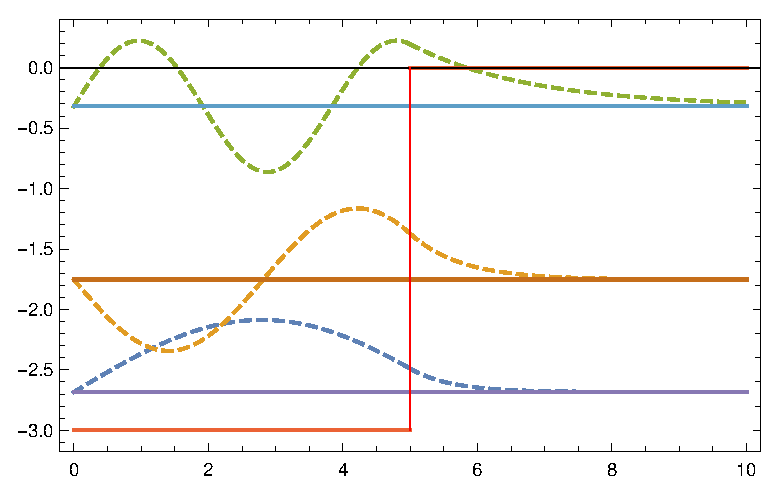
\includegraphics[width=0.42\textwidth]{PRSI.eps}%
		\label{fig:a}%
	}%
	\hfill%
	\subfloat[]{%
		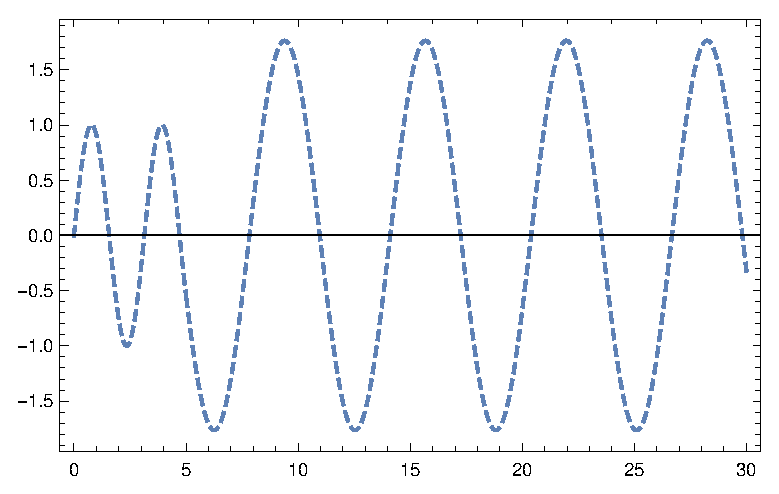
\includegraphics[width=0.42\textwidth]{SSSIPR.eps}%
		\label{fig:b}%
	}%
	\caption{\label{TRPR-Figure} (a) Pozo radial (línea sólida) para $R=5$, $V_0=3$ y sus correspondientes estados ligados (linea punteada). (b) Estado de dispersión correspondiente a $k=1$.}
\end{figure}

\subsection{Estados de dispersión.}

Para el espectro de dispersión, lo único que necesitamos es obtener el valor de las constantes de continuidad por medio de la fórmula (\ref{CSS}) para obtener la función de onda completa

\begin{equation*}
	u(k,r)=
	A
	\begin{cases}
	\sin(\sqrt{k^2 + V_0}r) & r \le R
	\\
	B e^{i k r} + C e^{- i k r} & R \le r
	\end{cases}
\end{equation*}

\begin{equation*}
	-C^{*}=B = e^{-i k R}[k \sin(\sqrt{k^2 + V_0}R)-i \sqrt{k^2 + V_0} \cos(\sqrt{k^2 + V_0} R)]
\end{equation*}

La figura \label{TRPR-Figure} muestra la gráfica de la función de onda para el estado de dispersión correspondiente al valor de la energía $k=1$. Procedemos a deformar el sistema por medio de la versión degenerada de la transformación de Darboux degenerada

\subsection{Sistema deformado}


Para la región de interacción, la función de transformación impar y su derivada con respecto a la energía están dadas por

\begin{eqnarray*}
u^{(i)}(q,r) &=& \sin(\sqrt{q^2 + V_0} r)
\\
\partial_q u^{(i)}(q,r) &=& \frac{q}{\sqrt{q^2 + V_0}} r \cos(\sqrt{q^2 + V_0} r),
\end{eqnarray*}

%donde el factor $ \frac{q}{\sqrt{q^2 + V_0}}$ al ser independiente a la posición, no contribuye al cálculo del nuevo sistema.%
El potencial deformado está dado entonces por la expresión analítica

\begin{equation*}
V_2 (r) =
\begin{cases}
-V_0 -  32 Q^2 \frac{Q r \cos(Q r) - \sin(Q r)}{(\sin(2 Q r) - 2 Q r)^2} \sin(Q r) & r < R
\\
32q^2\frac{[\sin{(qr)}-q(r+\gamma_0)\cos{(qr)}]\sin{(qr)}}{[\sin{2(qr)}-2q(r+\gamma_0)]^2} & R < r
\end{cases}
, \,\,\, Q^2 = q^2 + V_0 ,
\end{equation*}

la figura \ref{} muestra la gráfica de este potencial así como su discontinuidad en el punto de corte 

\begin{figure}
	\centering
	\subfloat[]{%
		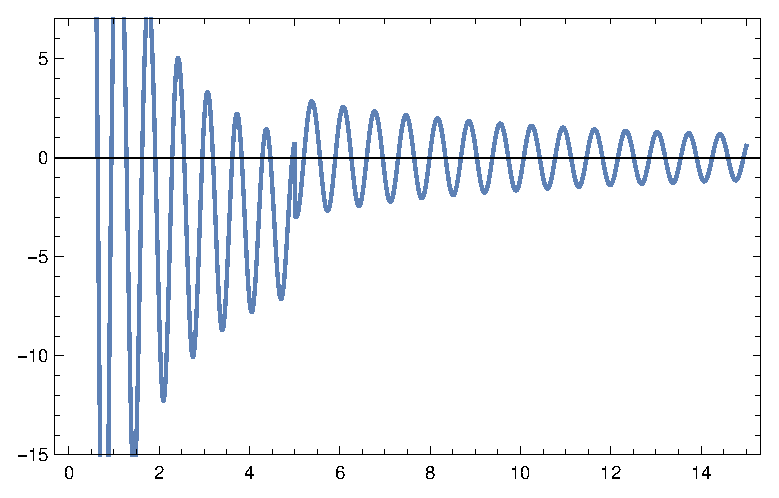
\includegraphics[width=0.42\textwidth]{PRPD.eps}%
		\label{fig:a}%
	}%
	\hfill%
	\subfloat[]{%
		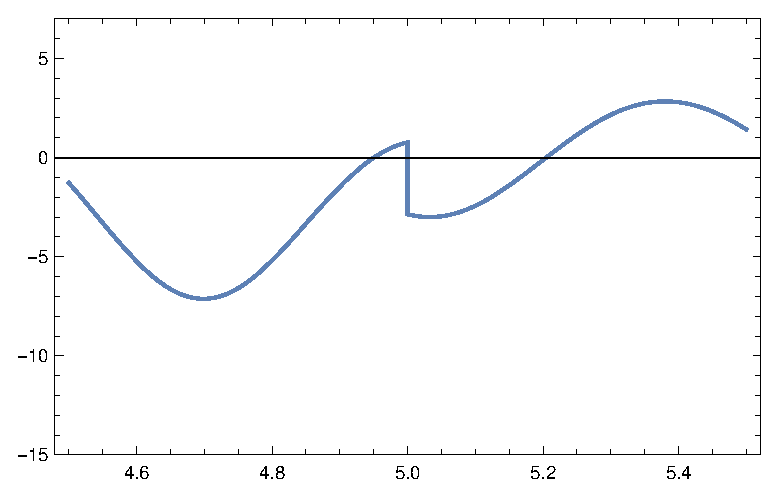
\includegraphics[width=0.42\textwidth]{PRDPD.eps}%
		\label{fig:b}%
	}%
	\caption{\label{TRPR-Figure} (a) Pozo radial para $R=5$, $V_0=3$ y sus correspondiente discontinuidad en el punto de corte.}
\end{figure}
 
 La función de onda  deformada para está región es entonces

\begin{eqnarray*}
	\psi^{(i)}(k,r) &=& \frac{\sin(K r)[(K^2 + Q^2)\sin(2 Q r)-2 (k^2 - q^2)K r] - 4 K Q \cos(K r)\sin^2(Q r)}{2Q r - \sin(2 Q r)},
	\\
	 K^2 &=& k^2 + V_0,\,\,\, Q^2 = q^2 + V_0
\end{eqnarray*}

Los estados ligados  y estados de dispersión del sistema deformado se muestran en la figura

\begin{figure}
	\centering
	\subfloat[]{%
		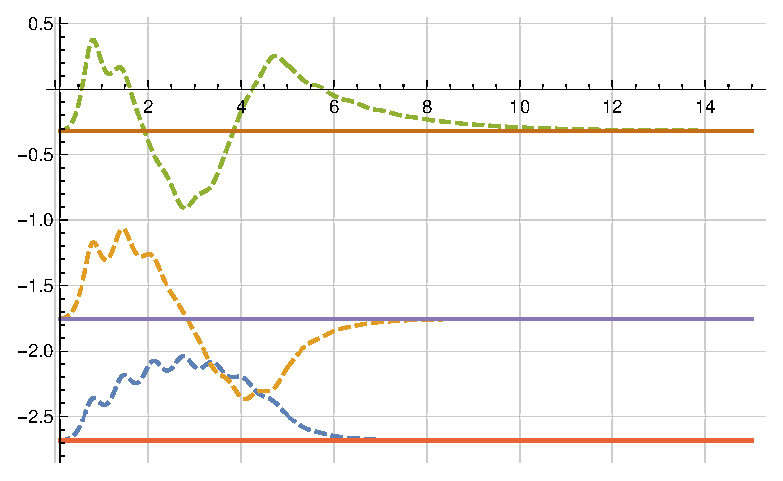
\includegraphics[width=0.42\textwidth]{PRDEL.eps}%
		\label{fig:a}%
	}%
	\hfill%
	\subfloat[]{%
		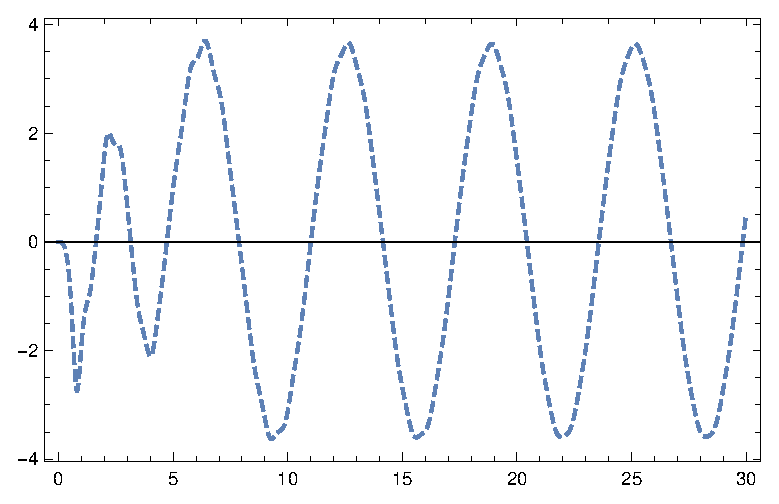
\includegraphics[width=0.42\textwidth]{EDSD.eps}%
		\label{fig:b}%
	}%
	\caption{\label{PRSD-Figure} (a) Estados ligados (linea punteada). (b) Estado de dispersión correspondiente a $k=1$ para el pozo radial deformado por medio de la transformación de Darboux degenerada para $\delta = 0$, $\gamma_0 = 1$, $V_0=3$, $R = 5$.}
\end{figure}



\section{Oscilador armónico truncado}

Como sistema inicial, se toma un oscilador armónico truncado cuyo umbral se encuentra en $V(r)=0$ y con punto de corte $r=R$

\begin{equation}
V(r)= \begin{cases}
r^2 - R^2 & r < R
\\ 0 & R < r \label{POAT}
\end{cases}
\end{equation}

En la región de interna, tememos un oscilador armónico con un offset $R$, por lo que la ecuación de Schrödinger se puede escribir de la forma

\begin{equation*}
-\frac{d^2 u^{(i)}}{dr^2} + r^2 u^{(i)}  = (k ^2 + R^2)u^{(i)} , \,\,\,\, k^2 = E
\end{equation*}

La forma más popular de resolver este tipo de sistemas es mediante el método de factorización, pues permite obtener de forma sencilla los estados ligados. Sin embargo, como en este caso el truncamiento genera un espectro que incluye un régimen continuo, es más conveniente realizar un mapeo a una ecuación hipergeométrica confluente, cuya solución es de la forma

\begin{equation}
	u^{(i)}(k,r) =A_i\,  _1F_1\left(a_k,\frac{1}{2};r^{2}\right) e^{-\frac{r^{2}}{2}} + B_i\,  _1F_1\left(a_k + \frac{1}{2},\frac{3}{2};r^{2}\right)re^{-\frac{r^{2}}{2}},\,\,\,\, a_k = \frac{1 - k^2 - R^2}{4} \label{OASC} 
\end{equation}

Donde la dependencia con respecto a la energía está contenida en el primer parámetro de $ _1F_1$, conocida como la función hipergeométrica confluente

\begin{eqnarray*}
\,  _1F_1\left(a, b ;r^{2}\right) = \sum_{n = 0}^{\infty}{\frac{(a)_n}{(b)_n}\frac{r^{2n}}{n!}},\,\,\, & (a)_n =
\begin{cases}
1 & a = 0
\\
\prod\limits_{k = 0}^{n-1} a + k & a \ne 0
\end{cases},
\end{eqnarray*}

Ya que se ha obtenido la función de onda para la región interna, se usará el método visto en la sección anterior en este sistema, empezando por construir los estados ligados correspondientes al potencial de partida.


\subsection{Estados ligados}

Siguiendo la metodología discutida en la sección anterior, la función de onda completa para los estados ligados correspondientes al oscilador armónico truncado $(\ref{POAT})$, es

\begin{equation*}
u(r)=A \begin{cases}
\,_1F_1\left(a_\kappa,\frac{3}{2};r^{2}\right)re^{-\frac{r^{2}}{2}} & r < R
\\\,_1F_1\left(a_\kappa,\frac{3}{2};b^{2}\right)R e^{R (\kappa -\frac{R}{2})} e^{-\kappa r} & R < r
\end{cases}
\end{equation*}

donde $k^2 = E < 0 \,:\, k = i \kappa,\, \kappa > 0 $.

Mientras que la condición de cuantización esta dada por la ecuación trascendental

\begin{equation*}
\frac{(3+\kappa^{2}-R^{2})R^{2}}{3}\, _1F_1\left(a+1,\frac{5}{2};R^{2}\right)-\left(R^{2}-b\kappa-1\right)\, _1F_1 \left(a,\frac{3}{2};R^{2}\right)=0.\label{TRHO-QR}
\end{equation*}

Esta ecuación es complicada de resolver analíticamente, por lo que es más conveniente buscar las raíces de forma numérica.La tabla \ref{TRHO-Table} muestra el espectro discreto (\ref{TRHO-QR}) para un valor específico del punto de corte $R$, mientras que la fugura \ref{TRHO-Figure} muestra dicho potencial y sus tres estados ligados. En la siguiente sección el espectro de dispersión será analizado.

\begin{table}
	\caption{\label{TRHO-Table} Espectro discreto del oscilador armónico truncado para $R=4$.}
	\begin{center}
		\begin{tabular}{ll}
			Estados Ligados & Energía\\
			
			Estado base & -12.999\\
			
			Primer estado excitado & -9.000\\
			
			Segundo estado excitado & -5.005\\
			
		\end{tabular}
	\end{center}
\end{table}

\begin{figure}
	\centering
	\subfloat[]{%
		\includegraphics[width=0.42\textwidth]{TRHO-Figure.eps}%
		\label{fig:a}%
	}%
	\hfill%
	\subfloat[]{%
		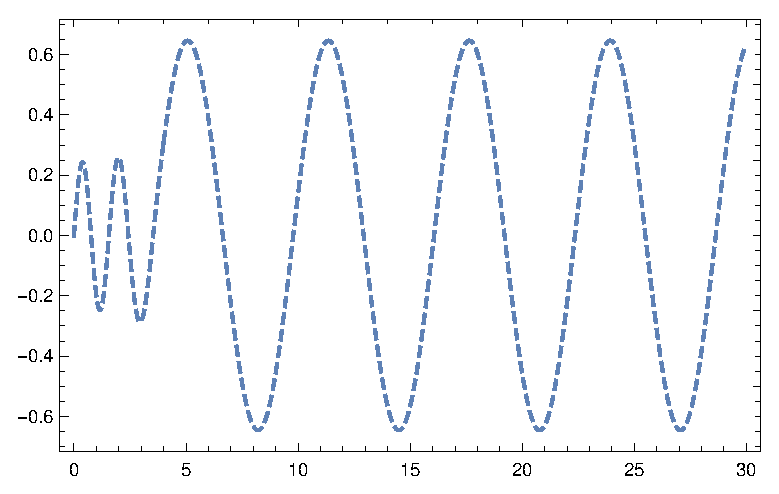
\includegraphics[width=0.42\textwidth]{Scattering.eps}%
		\label{fig:b}%
	}%
	\caption{\label{TRHO-Figure} (a) Oscilador armónico truncado (línea sólida) para $R=4$ y sus correspondientes estados ligados (linea punteada). (b) Estado de dispersión correspondiente a $k=1$.}
\end{figure}


\subsection{Estados de dispersión}

Si nos restringimos a los valores de $k^2 = E > 0$, y después de aplicar las condiciones de continuidad en el punto de corte, obtenemos las soluciones de la disoersión. La figura $\ref{TRHO-Figure}$ muestra la función de onda para el estado de la dispersión correspondiente a la energía $k = 1$.

\begin{eqnarray}
u_(r)=A\left\{
\begin{array}{cc}
\,\, _1F_1(a,3/2;r^2)\, r\, e^{-r^2/2}, & r\leq R  \\[0.2cm]
D(k,R)\, e^{ikr}+ D^{*}(k,R)\, e^{-ikr},&R<r   \label{TRHO-PsiS}
\end{array}
\right.
\end{eqnarray}
donde,
\small
\begin{eqnarray*}
	D(k) =
	\frac{A}{6k} e^{-\frac{1}{2}R(R+2ik)}\left\{3[i(R^{2}-1)+Rk^{2}]\, _1F_1\left(a_k ,\frac{3}{2};R^{2}\right)+iR^{2}(k^{2}+R^{2}-3)\, _1F_1\left(a_k+1,\frac{5}{2};R^{2}\right)\right\} 
\end{eqnarray*}

Ahora que hemos obtenido el espectro de dispersión, podemos utilizar una de estas soluciones como semilla para obtener un nuevo sistema por medio de la transformación de Darboux degenerada

\subsection{Oscilador armónico truncado deformado}

De acuerdo a el esquema planteado en la sección 3 y la forma de los estados de dispersión obtenida en esta sección, la función de transformación a utilizar para la transformación del oscilador armónico truncado debe ser de la forma

\begin{eqnarray}
u_T(r)=\left\{
\begin{array}{cc}
A_i \,\, _1F_1\left(a_{q},\frac{3}{2};r^{2}\right)re^{-\frac{r^{2}}{2}} , & r\leq R  \\[0.2cm]
A_e\,\sin{[qr+\delta]},&R<r   \label{DDT-TF}
\end{array}
\right.
\end{eqnarray}

donde,

\begin{equation}
a_q = \frac{3-q^2-R^2}{4}
\end{equation}

Ya que sólo necesitamos transformar la región interna, se requiere la derivada de la función hipergeométrica confluente respecto al primer argumento, pues en éste está contenida la dependecia con respecto a la energía. Con este fin, podemos escribir dicha función en forma de serie

\begin{equation*}
\, _1F_1\left(a_q,3/2;r^2 \right) = \sum_{n=0}^{\infty} \frac{(a_q)_n}{(3/2)_n} \frac{r^{2n}}{n!}.
\end{equation*}

Lo único que resta entonces es obtener la derivada $(a)_n$, conocido como símbolo de Pochhamer $citar$ o factorial descendiente. Esta derivada tiene la forma

\begin{equation*}
\frac{d}{da}(a)_n = (a)_n \left[ \frac{\Gamma'(a + n)}{\Gamma(a + n)}-\frac{\Gamma'(a)}{\Gamma(a)} \right]
\end{equation*}

donde $\Gamma(a)$ es la función gamma. Por lo tanto, la derivada de la función hipergeometrica confluente con respecto a la energía es

\begin{equation*}
\frac{d}{dq}\, _1F_1\left(a_q,3/2;r^2 \right) = \frac{da_q}{dq}\left \{ -\frac{\Gamma'(a_q)}{\Gamma(a_q)}\, _1F_1\left(a_q,3/2;r^2 \right)  + \sum_{n=0}^{\infty} \frac{\Gamma'(a_q + n)}{\Gamma(a_q + n)} \frac{(a_q)_n}{(3/2)_n} \frac{r^{2n}}{n!} \right \},
\label{DEFH}
\end{equation*}

ya que el primer término en los corchetes es proporcional a la misma función hipergeométrica, no contribuye al cálculo del nuevo sistema. Usando la formula para obtener el potencial deformado, en la región inerna éste está dado por la expresión analítica

\begin{equation*}
V^{(i)}(r)=r^{2}-R^{2} + 4+\frac{4}{r^2}-2\sum_{n=0}^{\infty}\frac{(a_{q})_{n}\Gamma'(a_{q}+n)}{(3/2)_{n}\Gamma(a_{q}+n)n!}\frac{d^{2}}{dr^{2}}\ln\left\{ {\rm W} \left[  _1F_1\left(a_{q},\frac{3}{2},r^{2}\right),r^{2n}\right]\right\}.\label{DDT-V<}
\end{equation*}

podemos observar que la singularidad en el origen está contenida en el cuarto término del lado derecho. La figura \ref{Figure vNWPot} muestra este potencial, así como su discontinuidad en el punto de corte. Lo siguiente es obtener las soluciones asociadas a la región interna del potencial, la cual está dada por la expresión analítica

\begin{equation}
\psi^{(i)}(k,r)=re^{-\frac{r^{2}}{2}}\frac{\sum_{m=0}^{\infty}\frac{(a_q)_{m}\Gamma'(a_{q}+m)}{(3/2)_{m}\Gamma(a_{q}+m)m!}{\rm W}\left[\, _1F_1\left(a_{q},\frac{3}{2},r^{2}\right),r^{2m},\, _1F_1\left(a_k,\frac{3}{2},r^{2}\right)\right]}{\sum_{n=0}^{\infty}\frac{(a_q)_{n}\Gamma'(a_{q}+n)}{(3/2)_{n}\Gamma(a_{q}+n)n!}{\rm W}\left[\, _1F_1\left(a_{q},\frac{3}{2},r^{2}\right),r^{2n}\right]}\label{Psi<}.
\end{equation}

Finalmente, podemos sustituir (\ref{Psi<}) en (\ref{FOPCADD}) y usar los métodos vistos en la sección anterior para obtener el espectro completo del sistema deformado, incluyendo un estado ligado en el continuo, lo que se muestra en la figura (\ref{DTHO})

\begin{figure}
	\centering
	\subfloat[]{%
		\includegraphics[width=0.41\textwidth]{Bound_States.eps}%
		\label{fig:a}%
	}%
	\subfloat[]{%
		\includegraphics[width=0.41\textwidth]{Scattering_DT.eps}%
		\label{fig:b}%
	}%
	\hfill%
	\subfloat[]{%
		\includegraphics[width=0.41\textwidth]{BIC.eps}%
		\label{fig:c}%
	}%
	\caption{\label{DTHO} (a) Scattering state of the Darboux deformed system for k=1, b=4, q=1.65996, $\delta=0$, $\gamma_0=1$. (b) The bound state in the continuum for the eigenvalue $k=q=1.65996$.}
\end{figure} 

Cabe resaltar que la regla de cuantización del sistema deformado es la misma que la del sistema inicial, lo que se muestra en la figura (\ref{})

\begin{figure}
	\centering
	\subfloat[]{%
		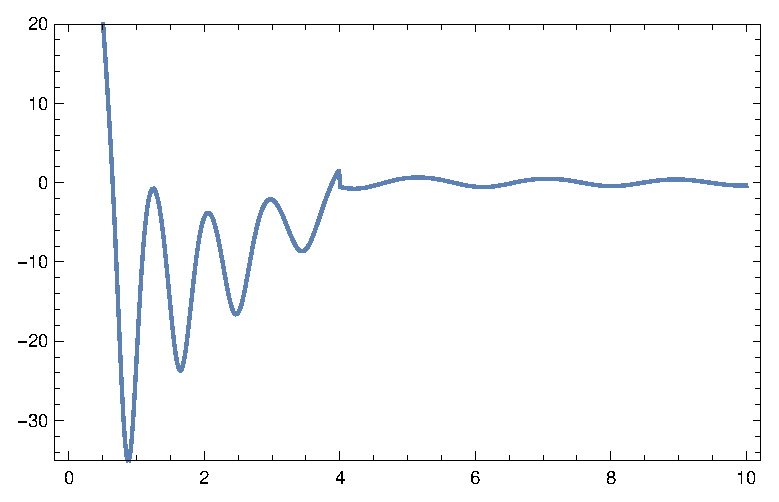
\includegraphics[width=0.41\textwidth]{Potential.eps}%
		\label{fig:a}%
	}%
	\hfill%
	\subfloat[]{%
		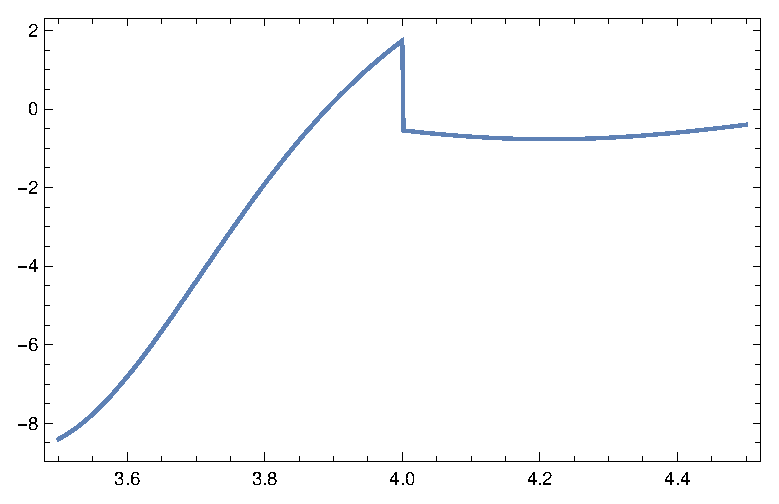
\includegraphics[width=0.41\textwidth]{Potential_discontinuity.eps}%
		\label{fig:b}%
	}%
	\caption{{\label{Figure vNWPot}} (a) Potencial Darboux - deformado para $q=1.65996$ y valores de los parámetros  $b=4$, $\delta=0$ y $\gamma_0=1$. (b) Discontinuidad del potencial en el punto de corte.}
\end{figure}

Por otro lado, el corrimiento de fase para el sistema perturbado se muestra en la figura \ref{}, donde se puede observar un incremento abrupto cerca de la energía del estado ligado en el continuo
\begin{figure}
	\centering
	\subfloat[]{%
		\includegraphics[width=0.41\textwidth]{CFOATD.png}%
		\label{fig:a}%
	}%
	\hfill%
	\subfloat[]{%
		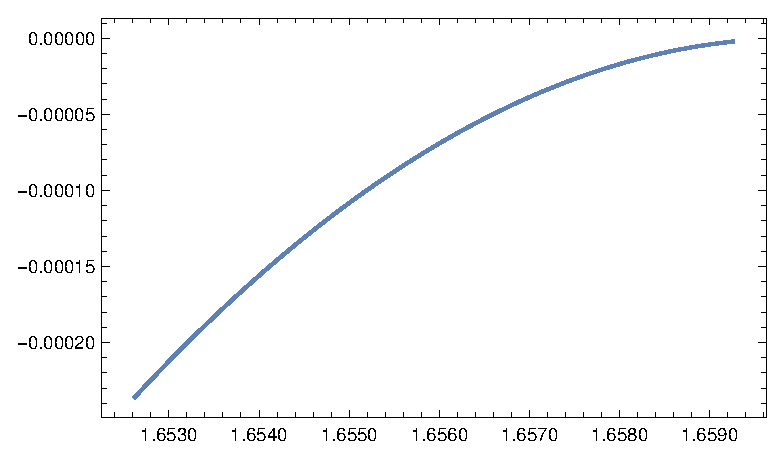
\includegraphics[width=0.41\textwidth]{SROATD.eps}%
		\label{fig:b}%
	}%
	\caption{{\label{Figure OHTD_BIC}} (a) Corrimiento de fase para un oscilador harmónico truncado deformado perturbado con $R = 4$, $\delta = 0$, $gamma_0$ = 1. (b) Seguimiento de la resonancia para el sistema perturbado desde $\lambda = 1$ a $\lambda = 0$}
\end{figure}

\section{Deformación parcial}
Ya que la definición del potencial de von Neumann - Wigner esta contenida en el comportamiento asintótico, la región interna no es relevante en este sentido. Por esta razón, en la presente sección se estudiará lo que ocurre al realizar la transformación de Darboux sólo en la región $R < r$. 

\begin{equation*}
	V(r) =
	\begin{cases}
		V^{(i)}(r) & r < R
		\\
		32q^2\frac{[\sin{(qr)}-q(r+\gamma_0)\cos{(qr)}]\sin{(qr)}}{[\sin{2(qr)}-2q(r+\gamma_0)]^2} & R < r
	\end{cases},
\end{equation*}

En este caso $V_< (r)$ es un potencial cuyas soluciones a la ecuación de Schrödinger son conocidas pero no provienen de la transformación de Darboux. Por ejemplo, para  el caso del oscilador armónico truncado $V_< (r) = r^2$. La función de onda completa en este caso es de la misma forma que $(\ref{FOGC})$ donde denotamos a la función en la región interna como $u^{(i)}$ para diferenciarla del caso de la transformación de Darboux completa

\begin{equation}
\psi_s(r)=\begin{cases}
A_i u^{(i)}(k,r) & r < R
\\\ B_e \psi^{+} + C_e \psi^{-} & R < r
\end{cases},\label{FOGCP}
\end{equation}

Siguiendo el mismo proceso de secciones anteriores, podemos obtener el valor de los coeficientes $B_e$ y $C_e$ para posteriormente escribir $\psi_s$ de manera conveniente


\begin{equation}
\psi_s(r)=A_i \begin{cases}
 u^{(i)}(k,r), & r < R
\\\ \frac{{\rm Im}\left\{W\left[ (k,r), \psi^{+}(k,r)\right]_{r=R}\psi^{-}(k,r)\right\}}{{\rm Im}\left\{\left[\psi^{-}(k,r)\frac{d}{dr}\psi^{+}(k,r)\right]_{r=R}\right\}},&R<r
\end{cases},\label{FOGCP}
\end{equation} 

Ya que el potencial tiene la forma asintótica $(\ref{FOAP})$, el posible estado ligado en el continuo se encuentra en el eigenvalor $E = q^2$, es decir, la energía correspondiente a la función de transformación para la región asintótica. Una vez más, podemos realizar el análisis en el límite $\sqrt{E} = k \to q$. La principal diferencia con respecto a lo realizado en las secciones anteriores, es que la función de onda en la región interna es diferente al caso trivial en dicho eigenvalor

\begin{equation*}
	u^{(i)}(q,r) \ne 0
\end{equation*}

Por lo tanto, no es necesaria la introducción de un polo a través de la variable $A_i$

\begin{equation*}
\lim_{k \to q}A_i u^{(i)}(k,r) = A_i u^{(i)}(q,r) 
\end{equation*}

Para la región $r < R$, por las propiedades $(\ref{PFL})$, podemos usar la regla de L'Hopital en el límite $k \to q$, en donde la ausencia del polo provoca que sólo se deba usar la regla dos veces. Sin embargo, el límite es de la misma forma, exceptuando el cambio del término $\partial^2_k \psi^{(i)} |_{k=q}$ por $u^{(i)}(q,R)$. 

\begin{equation*}
\lim_{k \to q} \frac{{\rm Im}\left\{W\left[u^{(i)}(k,r), \psi^{+}(k,r)\right]_{r=R}\psi^{-}(k,r)\right\}}{{\rm Im}\left\{\left[\psi^{-}(k,r)\frac{d}{dr}\psi^{+}(k,r)\right]\right\}_{r=R}} = \frac{f_n(q,R,r)}{f_d(q,R,r)}\,\,\,\,,
\end{equation*}


\begin{eqnarray*}
f_n(q,R,r)&=& W \left\{u^{(i)}(k,r), {\rm Re}[\psi^{+} (k,r)] \right\}_{k=q,r=R}  \,g_1(q,r)\\[0.2cm]
&+&2 \, W\left\{u^{(i)}(k,r), \partial_{k}{\rm Im}\left[\psi^{+}(k,r)\right]\right\}_{k=q,r=R}\, g_2(q,r)\\[0.2cm]
&+&\frac{2}{\gamma_0} \, W \left\{u^{(i)}(k,r),  \partial_{k}{\rm Re}\left[\psi^{+}(k,r)\right]\right\}_{k=q, r=R}\,g_3(q,r)\\[0.2cm]
&+& W \left\{u^{(i)}(k,r),\,\partial^2_k {\rm Im}\left[\psi^{+}(k,r)\right]\right\}_{k=q\,,r=R}\, g_3(q,r).
\end{eqnarray*}

Por lo tanto, la regla de cuantización en este caso es

\begin{equation*}
W[u^{(i)}(q,r),g_3(q,r)]_{r=R}=0
\end{equation*}

La figura ($\ref{FOATTDP}$) muestra el potencial creado por la transformación de Darboux parcial del oscilador armónico, la función de onda correspondiente al estado ligado en el continuo, su corrimiento de fase y el seguimiento de la correspondiente resonancia

\begin{figure}
	\centering
	\subfloat[]{%
		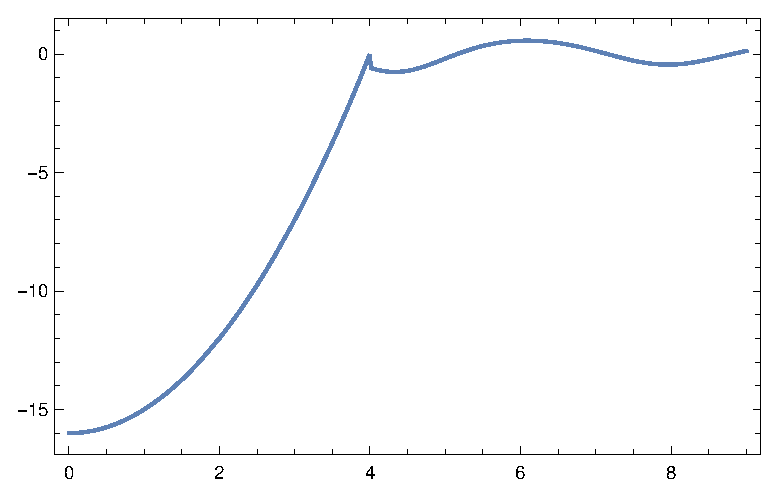
\includegraphics[width=0.41\textwidth]{POATTDP.eps}%
		\label{fig:a}%
	}%
	\hfill%
	\subfloat[]{%
		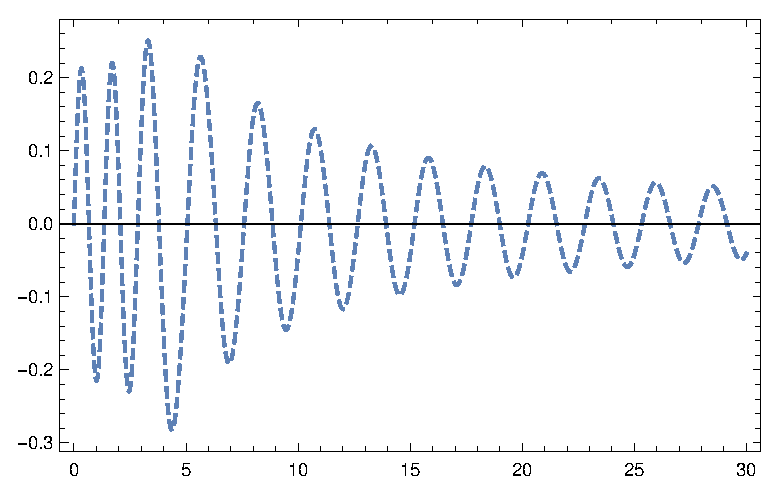
\includegraphics[width=0.41\textwidth]{BICTDPOAT.eps}%
		\label{fig:b}%
	}%
	\hfill%
	\subfloat[]{%
		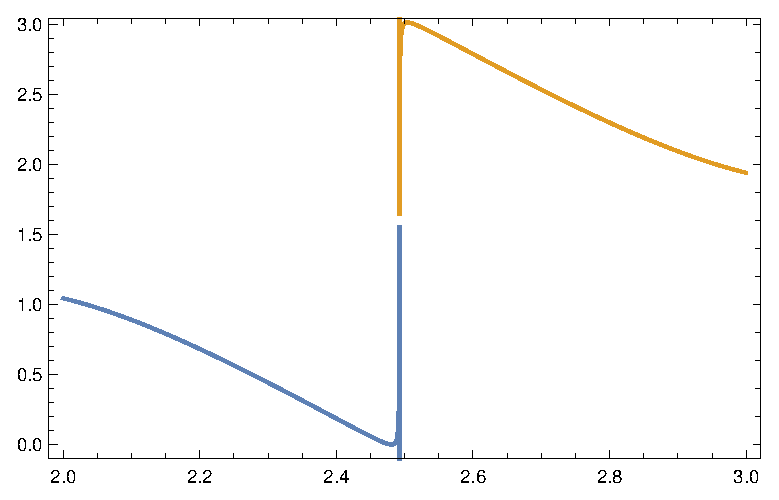
\includegraphics[width=0.41\textwidth]{CFOATDP.eps}%
		\label{fig:c}%
	}%
	\hfill%
	\subfloat[]{%
		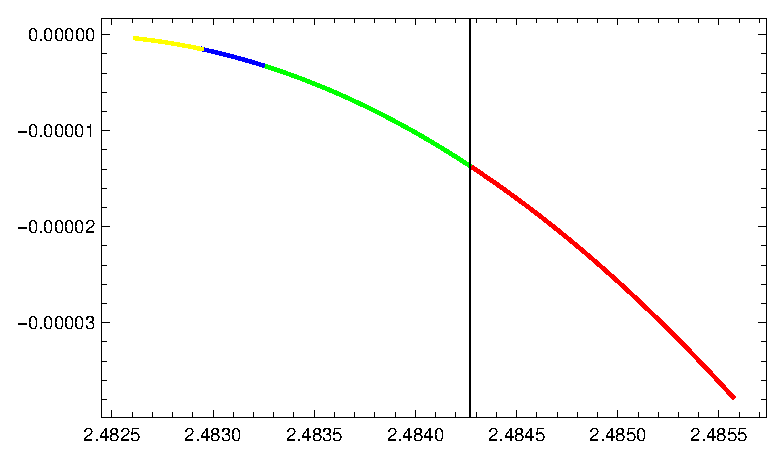
\includegraphics[width=0.41\textwidth]{SRDPOAT.eps}%
		\label{fig:d}%
	}%
	\caption{{\label{Figure-DPOA}} (a) Potencial Darboux - deformado parcialmente para $q=2.482279782872165$ y valores de los parámetros  $b=4$, $\delta=0$ y $\gamma_0=1$. (b) Estado ligado en el continuo correspondiente al potencial (c) Corrimiento de fase correspondiente a la resonanicia del sistema perturbado para $\lambda = 1$. Seguimiento de la resonancia para el sistema perturbado de $\lambda = 0.1$ a $\lambda = 1$ } \label{FOATTDP}
\end{figure}

